%=======================================================================================================================
%=======================================================================================================================
%===   Vorlage DA, MA, BA, SE, PS   (c) syssec 2017   ==================================================================
%===                                                  ==================================================================
%===   V2.1  290317                                   ==================================================================
%=======================================================================================================================
%=============================================================
%
\documentclass[11pt,twoside,openright,english]{klureport}
%
\usepackage[utf8]{inputenc}
\usepackage{graphicx}
\usepackage{amsmath,amsfonts,amsthm,color}
\usepackage{tabularx}
\usepackage{array}
\usepackage{setspace}
\usepackage{color}
\usepackage{listings}
\usepackage{tocbibind}
\usepackage{url}
\usepackage{multirow}
\usepackage{tabularx}
\usepackage[intoc]{nomencl}
\usepackage{titlesec}
\usepackage{ifthen}
\usepackage{fancyhdr}
\usepackage[T1]{fontenc}
\usepackage{lmodern}
\usepackage{float}
\usepackage{easyReview}
\usepackage{minted}
\usepackage{caption}

\newenvironment{code}{\captionsetup{type=listing}}{}

%-----------------------------------------------------------------------------------------------------------------------------------------
% Silbentrennung
%-----------------------------------------------------------------------------------------------------------------------------------------
% Bsp.: Bei-spiel --> Trennung Bei- spiel
%       dazu      --> keine Trennung
%
% !!!!!!!!!!!!!!!!
% !!! ANPASSEN !!!
% !!!!!!!!!!!!!!!!
\hyphenation{Bei-spiel dazu}

%-----------------------------------------------------------------------------------------------------------------------------------------
% Diverses Variablen
%-----------------------------------------------------------------------------------------------------------------------------------------
% !!!!!!!!!!!!!!!!
% !!! ANPASSEN !!! Umschaltung von DRAFT-Version auf FINAL-Version
% !!!!!!!!!!!!!!!! Vor dem Ausdruck für die gebundene Arbeit FINAL auf true setzen!
%
%                  Bis dahin nicht ersetzte Platzhalter (für Vorname, Nachname, Version, Datum, ...) führen dann zu einer Fehlermeldung!
%
\newboolean{FINAL}
\setboolean{FINAL}{false}

% !!!!!!!!!!!!!!!!
% !!! ANPASSEN !!! Sprache der Arbeit
% !!!!!!!!!!!!!!!!
% ENG = true  --> Englische Bezeichner und Abkürzungen --> Optionen bei \documentclass ÄNDERN!
%             --> \documentclass[11pt,twoside,openright,english]{klureport}
% ENG = false --> Deutsche  Bezeichner und Abkürzungen --> Optionen bei \documentclass ÄNDERN!
%             --> \documentclass[11pt,twoside,openright]{klureport}
%
\newboolean{ENG}
\setboolean{ENG}{true}

% !!!!!!!!!!!!!!!!
% !!! ANPASSEN !!! Geschlecht der Autorin bzw. des Autors
% !!!!!!!!!!!!!!!!
% FEMALE = true  --> Weibliche Bezeichner auf Titelseite
% FEMALE = false --> Männliche Bezeichner auf Titelseite
%
\newboolean{FEMALE}
\setboolean{FEMALE}{true}

% !!!!!!!!!!!!!!!!
% !!! ANPASSEN !!! Typ der wissenschaftlichen Arbeit
% !!!!!!!!!!!!!!!!
\def\TYPE{MA}
%
%  PS Proseminararbeit:    "Masterarbeit" --> "Proseminararbeit",
%                          "zur Erlangung des akademischen Grades Diplom-Ingenieur" --> entfällt
%  SE Seminararbeit:       "Masterarbeit" --> "Seminararbeit",
%                          "zur Erlangung des akademischen Grades Diplom-Ingenieur" --> entfällt
%  BA Bakkalaureatsarbeit: "Masterarbeit" --> "Bakkalaureatsarbeit",
%                          "zur Erlangung des akademischen Grades ..."
%  MA Masterarbeit:        "Masterarbeit" --> bleibt,
%                          "zur Erlangung des akademischen Grades Diplom-Ingenieur" --> bleibt

% !!!!!!!!!!!!!!!!
% !!! ANPASSEN !!! Individuelle Daten der Titelseite
% !!!!!!!!!!!!!!!!
\studname{Informatics}
\title{\ph {Training of the Language Model} \\
	\ph{PikabERT}}
\author{\ph{Corinna Grabner} \ph{BSc}}
\advisor{\ph {Assoc. Prof. Dipl-Ing. Dr. Konstantin Schekotihin}}
\version{\ph{0.01}}
%\date{\ph{Datum der Abgabe}}

%-----------------------------------------------------------------------------------------------------------------------------------------
% Automatisches Generieren der Daten für die Titelseite und andere Anpassungen
%-----------------------------------------------------------------------------------------------------------------------------------------
\newboolean{ZITAT}           % nicht ändern, flags werden automatisch gesetzt
\setboolean{ZITAT}{false}    %
\newboolean{DANK}            %
\setboolean{DANK}{false}     %

\ifthenelse{\boolean{ENG}}{
	\ifthenelse{\equal{\TYPE}{PS}}{
		\reporttype{Proseminararbeit}%{Proseminar Paper}
	}{
		\ifthenelse{\equal{\TYPE}{SE}}{
			\reporttype{Seminararbeit}%{Seminar Paper}
		}{
			\ifthenelse{\equal{\TYPE}{BA}}{
				\reporttype{Bachelorarbeit}%{Bachelor Thesis}
				\grade{Bachelor of Science}
				% \grade{Bakk. techn.} alter Studienplan
				\setboolean{DANK}{true}
			}{
				\ifthenelse{\equal{\TYPE}{MA}}{
					\reporttype{Masterarbeit}%{Master Thesis}
					\setboolean{ZITAT}{true}
					\setboolean{DANK}{true}
					\ifthenelse{\boolean{FEMALE}}{
						\grade{Diplom-Ingenieurin}
						%\grade{Master of Science} Informationsmanagement
					}{
						\grade{Diplom-Ingenieur}
						%\grade{Master of Science} Informationsmanagement
					}
				}{
					\reporttype{\ph{Type of work undefined!}}
				}
			}
		}
	}
}{
	\ifthenelse{\equal{\TYPE}{PS}}{
		\reporttype{Proseminararbeit}
	}{
		\ifthenelse{\equal{\TYPE}{SE}}{
			\reporttype{Seminararbeit}
		}{
			\ifthenelse{\equal{\TYPE}{BA}}{
				\reporttype{Bakkalaureatsarbeit}
				\grade{Bachelor of Science}
				% \grade{Bakk. techn.} alter Studienplan
				\setboolean{DANK}{true}
			}{
				\ifthenelse{\equal{\TYPE}{MA}}{
					\reporttype{Masterarbeit}
					\setboolean{ZITAT}{true}
					\setboolean{DANK}{true}
					\ifthenelse{\boolean{FEMALE}}{
						\grade{Diplom-Ingenieurin}
						%\grade{Master of Science} Informationsmanagement
					}{
						\grade{Diplom-Ingenieur}
						%\grade{Master of Science} Informationsmanagement
					}
				}{
					\reporttype{\ph{Typ der Arbeit undefiniert!}}
				}
			}
		}
	}
}
%-----------------------------------------------------------------------------------------------------------------------------------------
% Platzhalter
%-----------------------------------------------------------------------------------------------------------------------------------------
\ifthenelse{\boolean{FINAL}}{
	\newcommand{\ph}[1]{\end{document}}
}{
%   \newcommand{\ph}[1]{{\color[rgb]{1,0,0}\textbf{\uppercase{$<$#1$>$}}}}
\newcommand{\ph}[1]{{\color[rgb]{1,0,0}\textbf{$<$#1$>$}}}
}

%-----------------------------------------------------------------------------------------------------------------------------------------
% Generelle Daten für die Titelseite
%-----------------------------------------------------------------------------------------------------------------------------------------
%
% Altes Logo der Uni
%
%\university{\begin{center}
\includegraphics[width=0.5\textwidth]{Logos/UniLogo}\end{center}}

%
% Logo der TeWi (rechtsbündig) ohne \hfill linksbündig mit \begin{center}...\end{center} zentriert
%
% \university{\vspace*{-20mm}\hfill
\includegraphics[width=0.35\textwidth]{Logos/TeWiLogo}\vspace*{10mm}}
%
% KEIN LOGO MEHR!!!
%
% \university{\vspace*{-20mm}\hfill
\includegraphics[width=0.35\textwidth]{Logos/TeWiLogoBlue}\vspace*{10mm}}

\university{\vspace*{48pt}}

%
% \university{\vspace*{-20mm}\hfill
\includegraphics[width=0.35\textwidth]{Logos/TeWiLogoGreen}\vspace*{10mm}}

\universityname{Alpen-Adria-Universität Klagenfurt}
\city{Klagenfurt am Wörthersee}
\fakultaetname{Faculty of Technical Science}
\institute{Institut für Angewandte Informatik}
%\researchgroup{\ph {Name der Forschungsgruppe}}


%-----------------------------------------------------------------------------------------------------------------------------------------
% Kontaktadresse
%-----------------------------------------------------------------------------------------------------------------------------------------
% !!!!!!!!!!!!!!!!
% !!! ANPASSEN !!! eMail-Adresse der Autorin bzw. des Autors anpassen
% !!!!!!!!!!!!!!!!
%\ifthenelse{\boolean{ENG}}{
% \lowertitleback{
	%  In case of comments or problems, please contact the System Security Research Group
	% (\href{mailto:info@syssec.at}{info@syssec.at}) or the author (\href{mailto:peter@syssec.at}{\ph{email}}).
	%}
%}{
% \ifthenelse{\boolean{FEMALE}}{
	%  \lowertitleback{
		%   Bei Fragen, Problemen oder Anregungen kontaktieren Sie bitte die Forschungsgruppe Systemsicherheit
		%  (\href{mailto:info@syssec.at}{info@syssec.at}) oder die Autorin (\href{mailto:peter@syssec.at}{\ph{email}}).
		%}
	%}{
	% \lowertitleback{
		%  Bei Fragen, Problemen oder Anregungen kontaktieren Sie bitte die Forschungsgruppe Systemsicherheit
		% (\href{mailto:info@syssec.at}{info@syssec.at}) oder den Autor (\href{mailto:peter@syssec.at}{\ph{email}}).
		%}
	%}
%}

%-----------------------------------------------------------------------------------------------------------------------------------------
% Definitionen für diverse Verzeichnisse (Abkürzungsverzeichnis ,Inhaltsverzeichnis, ...)
%-----------------------------------------------------------------------------------------------------------------------------------------
\ifthenelse{\boolean{ENG}}{
\renewcommand{\abstractname}{Abstract}
\renewcommand{\contentsname}{Table of Contents}
\renewcommand{\nomname}{Table of Abbreviations}
\renewcommand{\lstlistlistingname}{Table of Listings}
\renewcommand{\lstlistingname}{Src.}

}{
\renewcommand{\abstractname}{Kurzfassung}
\renewcommand{\contentsname}{Inhaltsverzeichnis}
\renewcommand{\nomname}{Abkürzungsverzeichnis}
\renewcommand{\lstlistlistingname}{Quellcodeverzeichnis}
\renewcommand{\lstlistingname}{Src.}
}

\setlength{\nomlabelwidth}{.25\hsize}
\renewcommand{\nomlabel}[1]{#1 \hfill}
\setlength{\nomitemsep}{-\parsep}
\makenomenclature

%-----------------------------------------------------------------------------------------------------------------------------------------
% Definitionen für Überschriften
%-----------------------------------------------------------------------------------------------------------------------------------------
\titlespacing{\section}{0pc}{*3}{*0}[0pc]
\titlespacing{\subsection}{0pc}{*2}{-3pt}[0pc]
\titlespacing{\subsubsection}{0pc}{*1}{-6pt}[0pc]
\titlespacing{\paragraph}{0pc}{*3}{0.5em}

\titleformat{\chapter}{\normalfont\sffamily\LARGE\bfseries}{\thechapter}{0.5em}{}
\titleformat{\section}{\normalfont\sffamily\Large\bfseries}{\thesection}{0.5em}{}
\titleformat{\subsection}{\normalfont\sffamily\large\bfseries}{\thesubsection}{0.5em}{}
\titleformat{\subsubsection}{\normalfont\sffamily\bfseries}{\thesubsubsection}{0.5em}{}

%-----------------------------------------------------------------------------------------------------------------------------------------
% Diverse hilfreiche Kommandos und Definitionen
%-----------------------------------------------------------------------------------------------------------------------------------------
\newcommand{\topcaption}[1]{\caption{#1}\vspace*{3pt}}    % mehr Abstand zwischen Überschrift und Tabelle
\newcommand{\figcaption}[1]{\vspace*{-6pt}\caption{#1}}   % weniger Abstand zwischen Überschrift und Abbildung

\clubpenalty = 10000
\widowpenalty = 10000
\displaywidowpenalty = 10000

\renewcommand{\textfraction}{0.05}                        % ermöglicht Text auf Seiten mit großen Abbildungen (oder Tabellen, ...)

\setcounter{tocdepth}{2}                                  % Table Of Contents including Chapters, Sections and Subsections
\setcounter{secnumdepth}{2}                               % Counter up to Level 3: Chapter, Section, and Subsection

\raggedbottom                                             % Flattersatz am Seitenende --> konstante Abstände zwischen Absätzen

\linespread{1.1}                                          % etwas mehr als einfacher Zeilenabstand

%-----------------------------------------------------------------------------------------------------------------------------------------
% Definitionen für die Listing-Umgebung
%-----------------------------------------------------------------------------------------------------------------------------------------
\definecolor{hellgelb}{rgb}{1,1,0.8}
\definecolor{colKeys}{rgb}{0,0,1}
\definecolor{colIdentifier}{rgb}{0,0,0}
\definecolor{colComments}{rgb}{1,0,0}
\definecolor{colString}{rgb}{0,0.5,0}

\lstset {
float=hbp,%
basicstyle=\ttfamily\scriptsize,
%
% !!!!!!!!!!!!!!!!
% !!! ANPASSEN !!! Für SW-Druck ggfs. auskommentieren!
% !!!!!!!!!!!!!!!!
identifierstyle=\color{colIdentifier},
keywordstyle=\color{colKeys},
stringstyle=\color{colString},
commentstyle=\color{colComments},
backgroundcolor=\color{hellgelb},
%
columns=flexible,
tabsize=2,
frame=single,
extendedchars=true,
showspaces=false,
showstringspaces=false,
numbers=none,
numberstyle=\tiny,
breaklines=true,
breakautoindent=true,
captionpos=b,
language = Java,
frameround=tttt,
xleftmargin=1.5mm,
xrightmargin=1.5mm,
% linewidth=\textwidth
}

\lstloadlanguages{Java,XML}

\renewcommand{\lstlistoflistings}{\begingroup
\tocfile{\lstlistlistingname}{lol}
\endgroup}

%
% keine Liste der Listings im Inhaltsverzeichnis!
%
%\addtocontents{lol}{\protect\addvspace{10\p@}}%

%-----------------------------------------------------------------------------------------------------------------------------------------
% ein paar brauchbare neue Befehle
%-----------------------------------------------------------------------------------------------------------------------------------------
\newcommand{\changefont}[3]{\fontfamily{#1}\fontseries{#2}\fontshape{#3}\selectfont}

\newcommand{\bin}[1]{\text{°#1°}}
%\newcommand{\mycode}[1]{\changefont{cmtt}{m}{n}#1\normalfont}
%\newcommand{\mycode}[1]{\changefont{pcr}{b}{n}#1\normalfont}
%\newcommand{\mycode}[1]{\changefont{pcr}{m}{n}#1\normalfont}
%\newcommand{\inlinejavacode}[1]{{\ttfamily#1}}
%\newcommand{\inlinexmlcode}[1]{{\ttfamily#1}}
%\newcommand{\inlinejavacode}[1]{{\small\ttfamily#1}}
%\newcommand{\inlinexmlcode}[1]{{\small\ttfamily#1}}
\newcommand{\inlinejavacode}[1]{\lstinline[backgroundcolor=\color{white},basicstyle=\ttfamily\small]{#1}}
\newcommand{\inlinexmlcode}[1]{\lstinline[language=XML,backgroundcolor=\color{white},basicstyle=\ttfamily\small]{#1}}

\newcommand{\hex}[1]{\text{'#1'}}
\newcommand{\LE}{\ensuremath{\text{L}_\text{e}}}
\newcommand{\NE}{\ensuremath{\text{N}_\text{e}}}
\newcommand{\LC}{\ensuremath{\text{L}_\text{c}}}
\newcommand{\NC}{\ensuremath{\text{N}_\text{c}}}
\newcommand{\concat}{\ensuremath{||}}
\newcommand{\qq}[1]{``#1''}

\newcommand{\iso}[1]{ISO/IEC #1}
\newcommand{\isostand}[1]{ISO/IEC 7816-#1}

\newcommand{\ra}{\mbox{$\rightarrow$ }}

\newcommand{\zb}{z.B. }
\newcommand{\bzw}{bzw. }
\newcommand{\vgl}{vgl. }
\newcommand{\etc}{etc.}
\newcommand{\engl}[0]{engl. }
\newcommand{\gedankenstrich}{-- }

%-----------------------------------------------------------------------------------------------------------------------------------------
% Anpassung der Tabellenumgebung
%-----------------------------------------------------------------------------------------------------------------------------------------
\newcolumntype{L}[1]{>{\raggedright}p{#1}}
\newcolumntype{C}[1]{>{\centering}p{#1}}
\newcolumntype{R}[1]{>{\raggedleft}p{#1}}

\setlength{\extrarowheight}{2pt}

%=========================================================================================================================================
%=========================================================================================================================================
% BEGINN DES DOKUMENTS
%=========================================================================================================================================
%=========================================================================================================================================
\begin{document}

\frontmatter

\maketitle
\newpage
% !!!!!!!!!!!!!!!!
% !!! ANPASSEN !!! Zitat wird nur bei MA und DA eingebunden
% !!!!!!!!!!!!!!!!
\ifthenelse{\boolean{ZITAT}}{
	\begin{flushright}
		\textit{Zitat, falls gewünscht\\
			\begin{footnotesize}von wem?\end{footnotesize}}
	\end{flushright}
}{
}
\vspace*{28mm}


%-----------------------------------------------------------------------------------------------------------------------------------------
% Affidavit / Eidesstattliche Erklärung
%-----------------------------------------------------------------------------------------------------------------------------------------
% !!!!!!!!!!!!!!!!
% !!! ANPASSEN !!! Aktuelle Version der Studienabteilung nutzen! --> Siehe Upload-Formular der AAU!
% !!!!!!!!!!!!!!!!
\ifthenelse{\boolean{ENG}}{
	%
	% --> http://www.uni-klu.ac.at/studabt/downloads/affidavit.pdf (last visited 2018-01-19)
	%
	\begin{center}{\normalfont\sffamily\LARGE\bfseries Affidavit}\end{center} \vspace*{3mm}
	I hereby declare in lieu of an oath that
	\begin{itemize}
		\item[-] the submitted academic paper is entirely my own work and that no auxiliary materials have been used other than those indicated;
		\item[-] I have fully disclosed all assistance received from third parties during the process of writing the paper, including any significant advice from supervisors;
		\item[-] any contents taken from the works of third parties or my own works that have been included either literally or in spirit have been appropriately marked and the respective source of the information has been clearly identified with precise bibliographical references (e.g. in footnotes);
		\item[-] to date, I have not submitted this paper to an examining authority either in Austria or abroad and that
		\item[-] the digital version of the paper submitted for the purpose of plagiarism assessment is fully consistent with the printed version.
	\end{itemize}
	
	I am aware that a declaration contrary to the facts will have legal consequences.
	\vspace{2cm}
	
	\ph{Corinna Grabner, BSc} e.h. \hfill Klagenfurt, \ph{01.08.2021}
	
	\vspace*{2cm}
	\begin{center}
		\ph{Please check against the AAU version of this page or \\ 
			embed the AAU version!}
	\end{center}
	
	)
}{
	%
	% --> Am 19.1.2018 mit online verfügbarer Version abgeglichen
	%
	\begin{center}{\normalfont\sffamily\LARGE\bfseries Eidesstattliche Erklärung}\end{center} \vspace*{3mm}
	Ich versichere an Eides statt, dass ich
	\begin{itemize}
		\item[-] die eingereichte wissenschaftliche Arbeit selbstständig verfasst und keine anderen als die angegebenen Hilfsmittel benutzt habe,
		\item[-] die während des Arbeitsvorganges von dritter Seite erfahrene Unterstützung, einschließlich signifikanter Betreuungshinweise, vollständig offengelegt habe,
		\item[-] die Inhalte, die ich aus Werken Dritter oder eigenen Werken wortwörtlich oder sinngemäß übernommen habe, in geeigneter Form gekennzeichnet und den Ursprung der Information durch möglichst exakte Quellenangaben (z.B. in Fußnoten) ersichtlich gemacht habe,
		\item[-] die eingereichte wissenschaftliche Arbeit bisher weder im Inland noch im Ausland einer Prüfungsbehörde vorgelegt habe und
		\item[-] bei der Weitergabe jedes Exemplars (z.B. in gebundener, gedruckter oder digitaler Form) der wissenschaftlichen Arbeit sicherstelle, dass diese mit der eingereichten digitalen Version übereinstimmt.
	\end{itemize}
	Mir ist bekannt, dass die digitale Version der eingereichten wissenschaftlichen Arbeit zur Plagiatskontrolle herangezogen wird.
	
	Ich bin mir bewusst, dass eine tatsachenwidrige Erklärung rechtliche Folgen haben wird.
	
	\vspace{1cm}
	%
	% Bei der elektronischen Version ist es -- aus datenschutzrechtlichen Gründen -- nicht erforderlich, dass die eidesstattliche Erklärung
	% unterschrieben wird. Sie soll mittels Kürzel "e.h.", dieses ist dem Namen nachzustellen, elektronisch gezeichnet werden.
	%
	\ph{Vorname Nachname} e.h. \hfill \ph{Ort}, \ph{Datum}
	
	\vspace*{2cm}
	\begin{center}
		\ph{Vor der Abgabe                             \\
			mit Version der AAU abgleichen oder besser \\
			Version der AAU einbetten!}
	\end{center}
}

\newpage

%-----------------------------------------------------------------------------------------------------------------------------------------
% Danksagung
%-----------------------------------------------------------------------------------------------------------------------------------------
% !!!!!!!!!!!!!!!! Zumindest bei Bakkalaureats-, Masterarbeit sollten Sie bedenken, dass
% !!! ANPASSEN !!! einige Personen einige Mühen auf sich genommen haben, damit die Abgabe möglich war!
% !!!!!!!!!!!!!!!! Danksagung wird nur bei BA, MA und DA eingebunden
%
\ifthenelse{\boolean{DANK}}{
	\vspace*{28mm}
	\ifthenelse{\boolean{ENG}}{
		\begin{center}{\normalfont\sffamily\LARGE\bfseries Acknowledgements}\end{center} \vspace*{3mm}
	}{
		\begin{center}{\normalfont\sffamily\LARGE\bfseries Danksagung}\end{center} \vspace*{3mm}
	}
	Unser Dank gilt Raphael Wigoutschnigg, da diese Vorlage für wissenschaftliche Arbeiten der Gruppe Systemsicherheit
	(syssec) auf den LaTeX-Files seiner Diplomarbeit aufbaut.
}{
	\newpage
}

%-----------------------------------------------------------------------------------------------------------------------------------------
% Zusammenfassung
%-----------------------------------------------------------------------------------------------------------------------------------------
% !!!!!!!!!!!!!!!!!!!!!!!!!!!!!!!!!!!!!!!!!!!!!!!!!!!!!!!!!!!!!!!!!!!!!!!!!!!!!!!!!!!!!!!
% !!! ANPASSEN !!! ZUSAMMENFASSUNG MUSS ENTHALTEN SEIN UND DARF NICHT GELÖSCHT WERDEN !!!
% !!!!!!!!!!!!!!!!!!!!!!!!!!!!!!!!!!!!!!!!!!!!!!!!!!!!!!!!!!!!!!!!!!!!!!!!!!!!!!!!!!!!!!!
\begin{abstract}
	Infineon's Failure Analysis department examines the produced chips for errors in production and also deals with customer complaints. There are over 2,000 types of chips, which differ only minimally in layout. For the analysis, microscopes, lasers and X-Ray equipment is used. The department makes a very important contribution to the quality assurance of products at Infineon. If a product is not working properly, the resulting error code can be determined and the now called target product is sent to the failure analysis (FA) laboratory. Detection and localization of faults in semiconductors is a knowledge-intensive and tedious task. To increase the chances of success, an electrical engineer should be able to get all available information about the samples of similar past jobs. Various support systems used in Failure Analysis (FA), like databases, wikis, or file shares, often have this information stored as documents describing previous analysis reports of similar samples, best practices, specifications, customer reports, etc. However, accessing knowledge contained in these documents can be problematic, since in most cases, such support systems only provide rudimentary search functionality, like keyword matching. As a result, to find relevant information about jobs similar to the considered one, an engineer must query multiple systems, manually evaluate returned reports looking for similar characteristics, and asserting the value of each document for the current problem. \newline
	Modern Natural Language Processing methods (NLP) already showed their efficiency in various applications, including automatic translators, Recommender Systems or chatbots. Among these applications, text classification is one of the most promising to solve the FA search problem by automatically associating labels with a report denoting physical or electrical faults described in it, applied methods and tools, etc. The engineers can then use these labels to perform various tasks, like identifying similar jobs or getting statistics on possible faults, tools, or methods. \newline
	This is why one of the first applications of Artificial Intelligence (AI) tools at the FA laboratory of Infineon consisted on a classifier of the FA reports, using word2vec embeddings and clustering models, which satisfactory results. \newline
	With the apparition of more sophisticated tools in NLP during the last few years, the development of Transformer models until the publication of BERT, the results obtained by these models surpass anything utilized in previous times in almost every field where Transformers have been tested. 
	
	\vspace*{2cm}
	\ifthenelse{\boolean{ENG}}{
		\begin{center}
			{\normalfont\sffamily\LARGE\bfseries Zusammenfassung}
			\vspace{0.5em}
		\end{center}
		Die Fehleranalyseabteilung von Infineon untersucht die produzierten Chips auf Produktionsfehler und kümmert sich auch um Kundenreklamationen. Es existieren über 2.000 Chiptypen, die sich nur minimal im Layout unterscheiden. Für die Analyse werden Mikroskope, Laser und Röntgengeräte verwendet. Die Abteilung leistet einen sehr wichtigen Beitrag zur Qualitätssicherung der Produkte bei Infineon. Funktioniert ein Produkt nicht richtig, kann der resultierende Fehlercode ermittelt und an das FA-Labor gesendet werden. Das Erkennen und Lokalisieren von Fehlern in Halbleitern ist eine wissensintensive und langwierige Aufgabe. Um die Erfolgschancen zu erhöhen, sollte ein Elektroingenieur in der Lage sein, alle verfügbaren Informationen über ähnliche vergangene Jobs zu erhalten. Verschiedene Unterstützungssysteme, die in der Fehleranalyse (FA) verwendet werden, wie Datenbanken, Wikis oder Dateifreigaben, haben diese Informationen oft als Dokumente gespeichert, die frühere Analyseberichte ähnlicher Proben, Best Practices, Spezifikationen, Kundenberichte usw. beschreiben. Jedoch kann das Zugreifen auf das enthaltene Wissen in diesen Dokumenten problematisch sein, da solche Unterstützungssysteme in den meisten Fällen nur rudimentäre Suchfunktionen, wie z. B. Keyword-Matching, bereitstellen. Um relevante Informationen zu Jobs zu finden, die dem betrachteten ähnlich sind, muss ein Ingenieur daher mehrere Systeme abfragen, zurückgegebene Berichte manuell nach ähnlichen Merkmalen auswerten und den Wert jedes Dokuments für das aktuelle Problem bestätigen. \newline
		Moderne Methoden der Verarbeitung natürlicher Sprache (NLP) haben ihre Leistungsfähigkeit bereits in verschiedenen Anwendungen unter Beweis gestellt, darunter automatische Übersetzer, Recommender-Systeme oder Chatbots. Unter diesen Anwendungen ist die Textklassifizierung eine der vielversprechendsten, um das FA-Suchproblem zu lösen, indem Etiketten automatisch mit einem Bericht verknüpft werden, der darin beschriebene physikalische oder elektrische Fehler, angewandte Methoden und Werkzeuge usw. bezeichnet. Die Ingenieure können diese Etiketten dann zur Durchführung verwenden verschiedene Aufgaben, wie das Identifizieren ähnlicher Jobs oder das Abrufen von Statistiken über mögliche Fehler, Werkzeuge oder Methoden. \newline
		Aus diesem Grund bestand eine der ersten Anwendungen von Tools für künstliche Intelligenz (KI) im FA-Labor von Infineon in einem Klassifikator der FA-Berichte unter Verwendung von word2vec-Einbettungen und Clustering-Modellen, die zufriedenstellende Ergebnisse lieferten. \newline
		Mit der Entstehung immer ausgefeilterer NLP-Tools in den letzten Jahren, der Entwicklung von Transformer-Modellen bis zur Veröffentlichung von BERT, übertreffen die Ergebnisse dieser Modelle alles, was in früheren Zeiten in fast allen Bereichen, in denen Transformers getestet wurden, verwendet wurde.
	}{
		
}\end{abstract}

\newpage

\ifthenelse{\boolean{FINAL}}{}{{\color{blue}\vspace*{1cm}
		\begin{center}{\normalfont\sffamily\Large\bfseries Wichtige Hinweise zur vorliegenden LaTeX-Vorlage}\end{center}
		\begin{itemize}
			\item Diese Vorlage kann ohne Änderungen mittels PDFLaTeX von MikTeX compiliert werden. Daher müssen auch die
			Abbildungen als PDF vorliegen.
			\item Muss zur Compilierung aber LaTeX genutzt werden, da psfrag (oder Ähnliches verwendet wird),dann darf das Package
			hyperref nicht verwendet werden \ra Package hyperref (inkludiert am Beginn dieser Datei) auskommentieren und
			$\backslash$newcommand\{$\backslash$href\}[2]\{\#2\} definieren. Abbildungen müssen dann als eps vorliegen.
			\item Damit das Literaturverzeichnis erzeugt wird, muss ``bibtex thesis'' aufgerufen werden.
			\item Damit das Abkürzungsverzeichnis erzeugt wird, muss ``nomenclature.bat'' aufgerufen werden.
			\item Einige Dokumente die den Umgang mit LaTeX und diversen Packages beschreiben, finden Sie im Verzeichnis ``README''.
			\item Textstellen (wie Datumsangeben oder Nafkmen) die anzupassen sind, wurden teilweise mit Platzhaltern der Form
			\ph{Bechreibung} versehen! Nicht markierte Stellen der Titelseite, die gegebenenfalls anzupassen sind, umfassen
			\begin{itemize}
				\item Bezeichnung des Studiums und
				\item Name der betreuenden Assistentin bzw. des betreuenden Assistenten.
			\end{itemize}
			\item Bitte Sicherstellen, dass die Titelseite und die Eidesstattliche Erklärung der aktuellen Fassung der AAU entsprechen. Die zugehörigen Seiten können auch auf der Upload-Seite der AAU erzeugt und in dieses Dokument eingebunden werden.
			\item Vor dem Ausdruck für die gebundene Masterarbeit ist die boolesche Variable ``FINAL'' (siehe Zeile 49 in dieser Datei)
			auf ``true'' zu setzen! Nicht ersetzte Platzhalter -- das sind Kommandos der Form $\backslash$ph\{\ldots\} -- werden dann beim Aufruf von PDFTex zu einer Fehlermeldung führen.
			\item Die aktuelle Version dieses Dokuments finden Sie auf der Website des Instituts für Angewandte Informatik \url{https://www.aau.at/en/ainf/teaching/templates}.
		\end{itemize}
}}

%-----------------------------------------------------------------------------------------------------------------------------------------
% Inhaltsverzeichnis
%-----------------------------------------------------------------------------------------------------------------------------------------
\newtableofcontents

%-----------------------------------------------------------------------------------------------------------------------------------------
% einzelne Kapitel
%-----------------------------------------------------------------------------------------------------------------------------------------
\mainmatter   % arabic page numbering

\chapter{Introduction} \label{chapter:introduction}

Infineon technologies Austria is one of the leading semiconductor companies worldwide. With around 4,820 employees, the company makes an important contribution to shaping the digital and networked future. Through the development of microelectronics and their constant improvement, Infineon enables efficient energy management, intelligent mobility and secure, seamless communication. \newline

\section{Motivation}
Detection and localization of faults in semiconductors is a knowledge-intensive and tedious task. To increase the chances of success, an electrical engineer should be able to get all available information about the samples of similar past jobs. Various support systems used in Failure Analysis (FA), like databases, wikis, or file shares, often have this information stored as documents describing previous analysis reports of similar samples, best practices, specifications, customer reports, etc. However, accessing knowledge contained in these documents can be problematic, since in most cases, such support systems only provide rudimentary search functionality, like keyword matching. As a result, to find relevant information about jobs similar to the considered one, an engineer must query multiple systems, manually evaluate returned reports looking for similar characteristics, and asserting the value of each document for the current problem. Furthermore, the report corpus includes a quantity of over one million documents, which means a long search time if you are looking for a specific topic. These procedure is depicted in Figure \ref{fig:fa_process}

\begin{figure}[H]
	\centering
	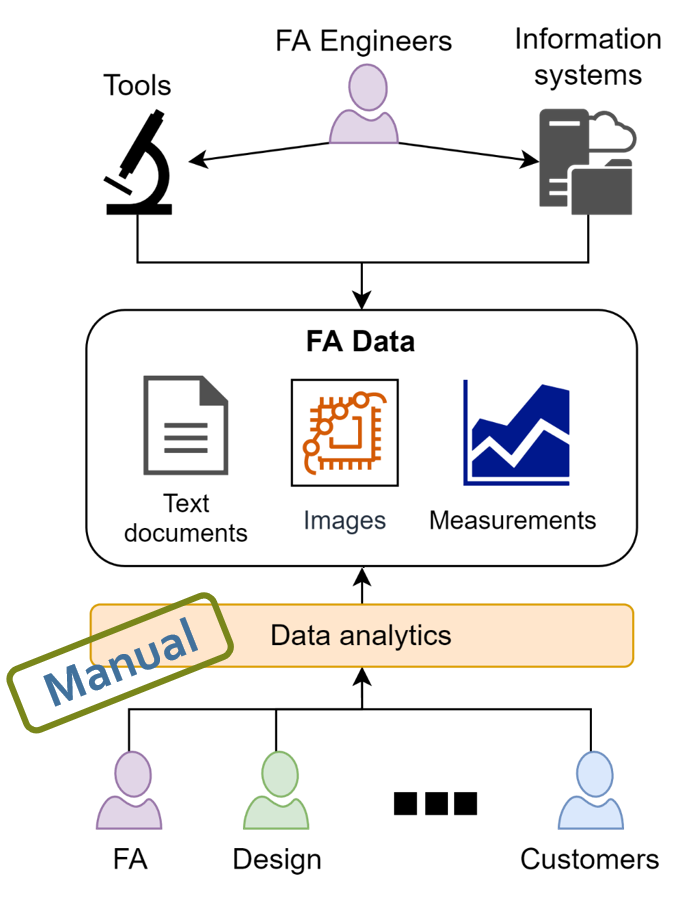
\includegraphics[width=0.3\textwidth]{figures/fa_process.png}
	\caption{FA Analysis Process}
	\label{fig:fa_process}
\end{figure}

In order to accelerate this process of troubleshooting and to make it easier to find similarities between past and new jobs, the integration of artificial intelligence in the failure analysis process is suitable. Integrating AI into Infineons failure analysis could look like in Figure \ref{fig:ai_process} where AI infrastructures are used to load and process ressources and help not only FA employees, but all Infineon employees and customers to better understand the existing data through appropriate processing and to be able to use it in a targeted manner.

\begin{figure}[H]
	\centering
	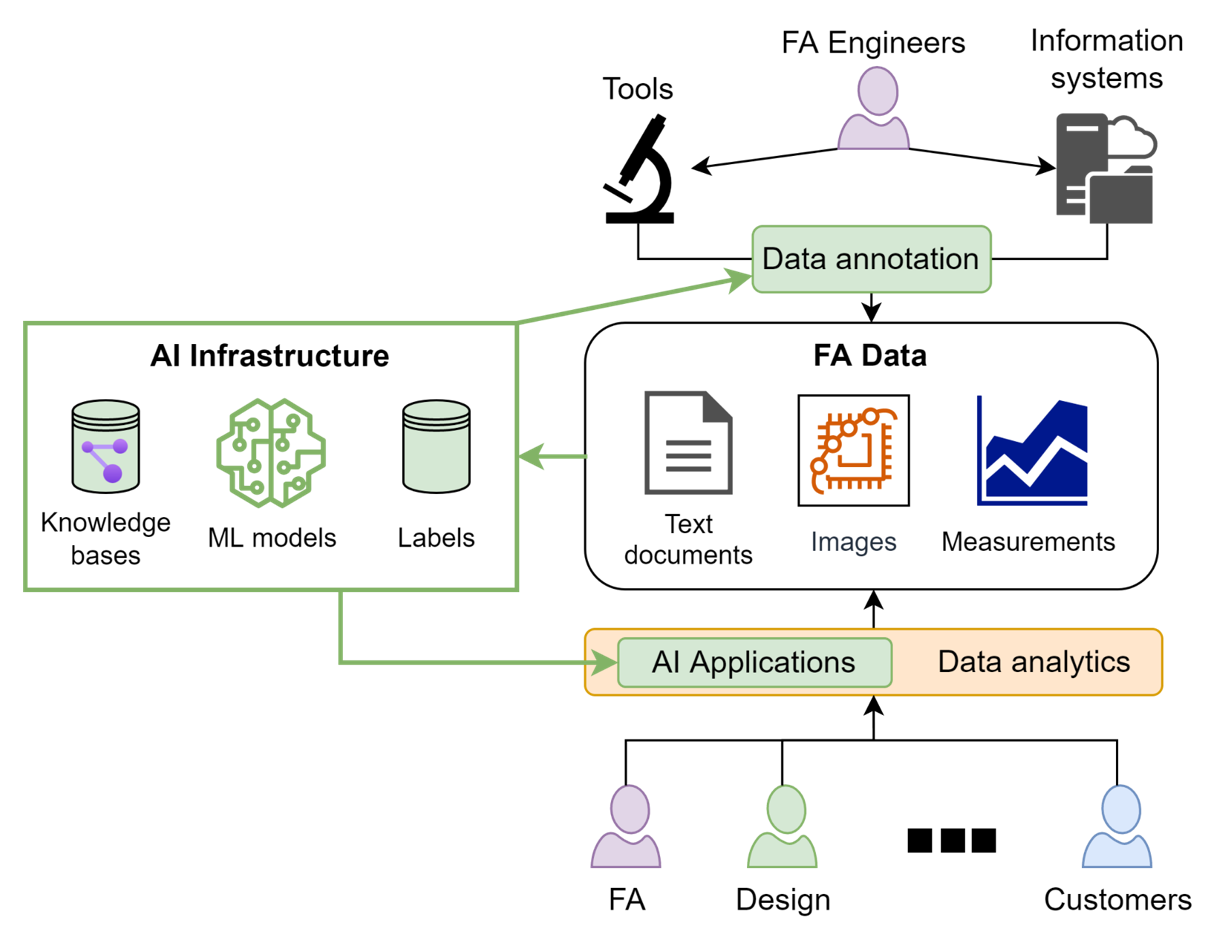
\includegraphics[width=0.6\textwidth]{figures/ai_process_idea.png}
	\caption{FA Analysis Process with AI Integration}
	\label{fig:ai_process}
\end{figure}

Modern Natural Language Processing methods (NLP) already showed their efficiency in various applications, including automatic translators, Recommender Systems or chatbots. Among these applications, text classification is one of the most promising to solve the FA search problem by automatically associating labels with a report denoting physical or electrical faults described in it, applied methods and tools, etc. The engineers can then use these labels to perform various tasks, like identifying similar jobs or getting statistics on possible faults, tools, or methods. \newline
This is why one of the first applications of Artificial Intelligence (AI) tools at the FA laboratory of Infineon consisted on a classifier of the FA reports. To support the classifier and improve performance as best as possible, a language model is trained on in-domain text data as shown in Figure \ref{fig:fa_bert_process}. The model should support engineers during the analysis and report writing process.

\begin{figure}[H]
	\centering	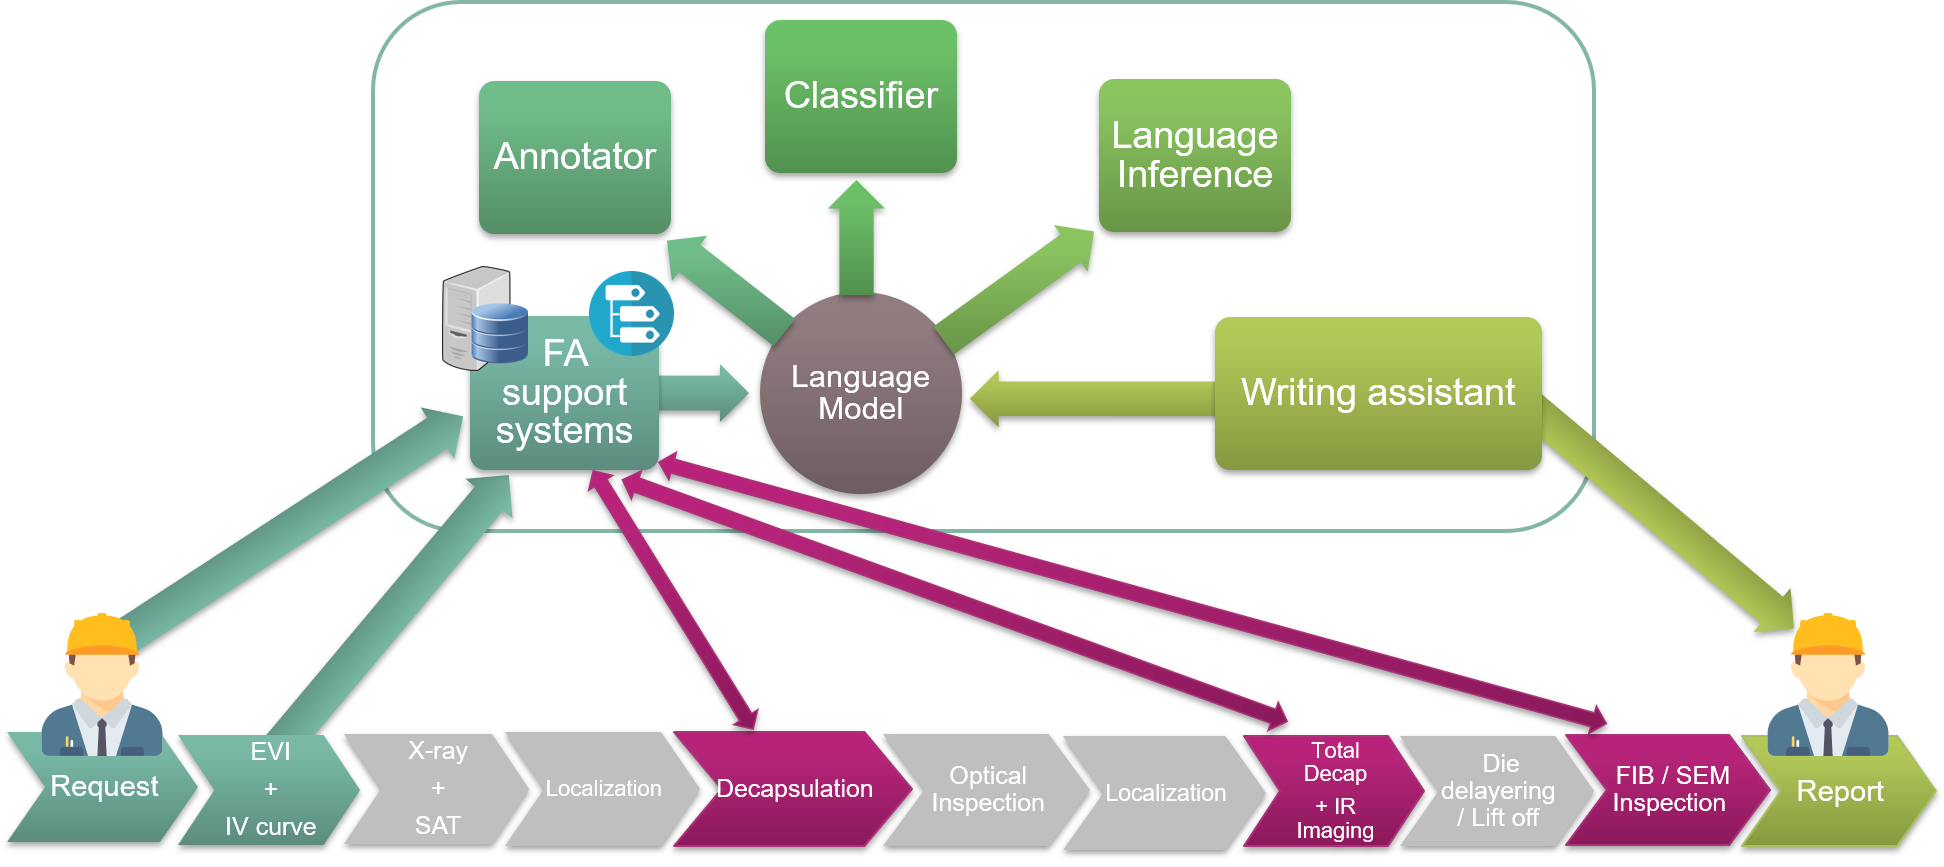
\includegraphics[width=1\textwidth]{figures/fa_bert_process.png}
	\caption{FA-BERT Integration into FA Analysis Prozess}
	\label{fig:fa_bert_process}
\end{figure}

After receiving a in-domain trained language model it can be used for several downstream tasks like classification of electrical and physical failures, improving the classification results by segmenting FA texts according to their topic, Named Entity Recognition (NER) were the model will be integrated in the production environment for automated annotation of FA reports or Natural Language Inference (NLI) tasks for question answering and information retreival.

\section{Problem Description}
The goal of this project is to develop a FA report classifier with a BERT model.
In order to do so, the task has been divided into two phases: \newline
First, we have developed a Language Model based on the state-of-the-art model BERT. Therefore we had to consider our specific domain and select the most appropriate model for our domain. Since many successors of BERT have been developed but none of them aimed at the electrical domain, we had to select a model as close as possible to our field of study in order to achieve a satisfying performance later. \newline
Second, we focused on defining the structure of the classifier, which consisted on the BERT network and additional classification layers. To test the results, we have defined a series of classification problems based on the FA reports. \newline
Given the nature of this project the two phases were developed in parallel so the joint performance hasn't been tested yet. \newline

\section{Research Questions}
This thesis will address the following research questions:
\begin{itemize}
	\item What kind of BERT models already exist and which one to choose as an entrypoint for training?
	\item What data should be used for further training and how to collect it?
	\item How to train and evaluate the resulting model?
\end{itemize}

The following chapters in this thesis will cover the research questions described above. Before that, as a basis for the content that follows, some terms and topics related to natural language processing will be discussed.

\section{Contributions}
\textbf{RQ1: What kind of BERT models already exist and which one to choose as an entrypoint for training?} \newline
In order to fulfill the goal of developing an innovative language model trained on the semiconductor domain, it was necessary to find an existing language model which has already been trained on english text similar to electrical engineering or semiconductor topics. With this language model to use as entry point for our training, we assumed it would be easier to achieve our desired goals. 
After extensive search and research, we found possible candidates for the model entry point. One of the largest BERT models is Med-BERT, which has been trained on medical and biomedical documents. Unfortunately, this model is not suitable as a starting point for our training, since words in medical texts are very similar to those in semiconductor texts but have a different semantic meaning. Because of this, the model can become "confused" when trying to understand the text. Other promising models are SciBERT and S2ORC-SciBERT. Both models are trained using scientific, english texts, with the training corpus consisting of chemistry, physics, but also mainly medical topics. In contrast to SciBERT, S2ORC-SciBERT has a slightly larger vocabulary and was also trained on a larger data set, which also includes topics such as computer science and engineering. \newline
After some evaluation processes on error analysis reports, S2ORC-SciBERT could be chosen as the entry point. The performance of S2ORC-SciBERT is slightly better than that of SciBERT.

\textbf{RQ2: What data should be used for further training and how to collect it?} \newline
To further train the language model entrypint on a domain specific dataset to achieve the desired results, the specific dataset had to be collected and transformed into a shape which allows to train a BERT based language model. To collect the domain specific texts, we used \textit{GoogleScholar}, \textit{SemanticScholar} and \textit{IEEE} to download as many papers as possible. Also we used parts of the S2ORC dataset and filtered for texts with the topics chemistry, physics, computer science, mathematical science and engineering. After collecting the papers, the raw text had to be extracted. Therefore we were allowed to use a text extractor tool developed by Infineon collegues in Bangalore and did not had to develop it on our own. The raw text had been saved in csv files and could be loaded to create a okenized dataset ready for training. In total the training data frame included 1 783 789 rows which is about 10GB of data.


\textbf{RQ3: How to train and evaluate the resulting model?} \newline
As a training method we decided to choose the most common way of how to pretrain a BERT-based model: using Masked Language Modeling. This technique had already been used for training the original BERT model and will now also been used in an adapted way for our training experiments. In order to achieve a satisfying result, we wanted our model to understand the FA reports as good as possible. With the whole-word-masking technique, which is an adaption of the traditional masked language modeling algorithm, we achieved a lower loss during training. The evaluation of the final model on the FA report job summaries show, that our trained model has a better understanding of the texts than the initial model.
\chapter{Literature Review} \label{chapter:literaturereview}

\section{Natural Language Processing}
\alert{Communication and the sharing of knowledge is an essential part of human society. History has shown that the best way to transmit knowledge is in writing. It is not difficult for a person to learn to read and to understand the context in texts. For computers, this task is much more difficult. Natural Language Processing (NLP) is a subfield pf Artificial Intelligence (AI) which deals with teaching computers to understand and interpret human language and has emerged in 1940. The initial need of NLP was the translation from one language into another which was used during the second world war. Nowadays it is widely used in health care, spam detection, sentiment and cognitive analysis. NLP also provides computers with the ability to read text, hear speech, and communicate with humans. Every person had contact with a NLP device at least once in their life. The best example everyone might know are personal assistants like Siri or Alexa. These are applications which work with NLP and have learned to communicate with humans and nearly seem humanely.\newline
Generally speaking, NLP breaks down language into shorter, more basic pieces, called tokens (words, periods, etc.) which get saved as vectorial representations. The technique of mapping words to real vectors is called word embedding. To understand the relationships of the tokens, the model gets trained by predicting some hidden part of the text using some other part of their surrounding text. One way to calculate the representations of the vectors is the method \textit{Word2Vec}. Until BERT has emerged, Word2Vec was the most common technique to create word embeddings. It is a two-layer neural network which processes text and turns it into a numerical form that can be understand by deep neural networks. Given enough data, Word2vec can make highly accurate guesses about a word’s meaning based on past appearances. Those guesses can be used to establish a word’s association with other words. The diference between Word2Vec and BERT will be covered in Section \ref{bert}}.

\section{Text Representation}

\subsection{Tokenization}
Texts cannot be processed by ML models directly. Tokenization is a method that transforms sequences of characters into a sequence of integers. As an example we can take the sentence: \newline

\centerline{"This is a cat."} 

A tokenization transforms this sentence into [‘This’, ‘is’, ‘a’, cat’]. Punctuations will be removed. This step is important to help the model understanding the meaning of a text. The model can
\begin{itemize}
	\item Count the number of words in the text
	\item Count the frequency of the word, that is, the number of times a particular word is present
\end{itemize} 

In modern LMs, tokenizers are trained together with the model to identify the best possible transformations, which can happen on both word and sub-word levels. The set of obtained tokens determines the vocabulary of an LM. If a word appears in the vocabulary of LM, it can be represented as a vector in the target space. Otherwise, a word is split into parts until each of them can be mapped to a set of tokens from the vocabulary. In the worst case, a word is split into individual letters. Such splitting may significantly reduce the quality of word embeddings in the vector space, thus reducing the quality of features extracted for the classification layers of a network. Therefore, it is essential either to select an LM whose vocabulary provides good coverage of the main terms used in an application domain or to extend the vocabulary of an LM with these terms and fine-tune it on domain-specific texts. 

\subsection{Bag of Words}
Bag of Words is a method for simplifying the representation of documents and the importance of the words they contain which is used in NLP and Information Retreivel (IR). Here the sentences in the documents are divided into their individual words and counted. The resulting object contains a list of the contained words and the number of their occurrences. It is called a “bag” of words, because any information about the order or structure of words in the document is discarded. The model is only concerned with whether known words occur in the document, not where in the document. We will describe the concept of bag-of-words with the following example: The below snippet contains the first few lines of \alert{the book "A Tale of Two Cities" by Charles Dickens. Different example?}


\textit{
\centering	
It was the best of times,\\
it was the worst of times,\\
it was the age of wisdom,\\
it was the age of foolishness, \\
}

In this example, each line will be treated as an individual document. The model vocabulary is containing the following 10 words:
\begin{itemize}
	\item “it”
	\item “was”
	\item “the”
	\item “best”
	\item “of”
	\item “times”
	\item “worst”
	\item “age”
	\item “wisdom”
	\item “foolishness”
\end{itemize}

Using this vocabulary, vector representations can be created for any document. For this purpose, a suitable scoring method must be chosen. The scoring method can be binary scoring or frequencies. Table \ref{tab:scoring} is showing an example of the resulting vector representations for a document which contains the first line in our example.

\begin{table}[H]
	\centering
	\begin{tabular}{ll}
		\hline
		\textbf{Scoring Method} & \textbf{Resulting Vector Representation}                                         \\ \hline
		Binary & [1, 1, 1, 1, 1, 1, 0, 0, 0, 0] \\ \hline
		Frequencies & [1, 1, 1, 1, 1, 1, 0, 0, 0, 0] \\ \hline
	\end{tabular}
	\caption{Example of scoring methods}
	\label{tab:scoring}
\end{table}

\subsection{Term Frequency - Inverse Document Frequency}
Term Frequency - Inverse Document Frequency (TF-IDF) is a statistical measure to determine how important a word is within a document. It determines not only how often a word appears in a single document, but also how often it appears in the entire document corpus. Very common words like "this" or "and" get a lower score, even though they occur often, because they are not important for the context of a document. This will be determined by comparing the occurrence of these words among the documents. This strategy is often used in NLP for text analysis. For example, in a failure analysis report, a word like failure would get a high score. By using other important words, the report could be automatically assigned to a certain failure type and thus classified. \\
TF-IDF for a word in a document is calculated by multiplying the term frequency and the inverse document frequency.

\begin{align}
	tf idf (t, d, D) &= tf(t, d) * idf(t, D)
\end{align}
Where
\begin{align}
	tf (t, D) &= log(1 + freq(t, d)) \\
	idf(t, D) = log(N/count(d E D, t E d))
\end{align}

The term frequency \textit{tf} is either a simple count of instances a word appears in a document or it can be adjusted by taking the length of the document to account. The calculation can be seen in (2.3) where \textit{t} is the term and \textit{D} the document to analyse. The inverse document frequency \textit{idf} is determined accross the document corpus. The closer this metric is to zero, the more common a word is. The calculations can be seen in (2.4) where \textit{N} is the number of documents.

\subsection{Word Embeddings}
A machine is not able to process text in its raw form. Word embedding is a technique were words are transformed into a numerical representation, a vector. This embedding is then fed into machine learning models. The simplest embedding technique is one hot encoding which would look as in Table \ref{tab:onehot}.

\begin{table}[H]
	\centering
	\begin{tabular}{ll}
		\hline
		\textbf{Word} & \textbf{Vector Representation} \\ \hline
		have & [1, 0, 0, 0, 0, 0, ... 0]\\ 
		a    & [0, 1, 0, 0, 0, 0, ... 0]\\ 
		good & [0, 0, 1, 0, 0, 0, ... 0]\\ 
		day  & [0, 0, 0, 1, 0, 0, ... 0]\\ \hline
	\end{tabular}
	\caption{One Hot Encoding Example}
	\label{tab:onehot}
\end{table}

Because the vector representations may get quite large with one hot encoding, there is the need of more effective encoding techniques.

\subsubsection{Word2Vec Architecture}
Word2vec is not a singular algorithm, it is a family of model architectures and optimizations that can be used to learn word embeddings from large datasets. The strength of Word2Vec lies in assigning similar vectors to words with similar meanings. 






\section{Masked Language Modelling}

\subsection{Transformer}
The transformer in the field of NLP is a new architecture which is able to solve sequence-to-sequence tasks while handling dependencies in the text. Transformers basically consist of an encoder and a decoder. The encoder reads the input text and the decoder produces a prediction. Transformers work in small increments. In each step, an attention mechanism is applied to understand the relationships between the words in a sentence, regardless of their positions. Both encoder and decoder sections of transformer are a stack of 6 identical layers of multi-head attention and feed forward sublayers. \alert{Each sublayer takes a residual connection from its previous inputs, adds it to the sub layer output and normalises it to produce final output of the sub layer. To allow for residual addition, all sub-layers produce an output of dimension 512.} The architecture is depicted in Figure \ref{fig:transformer}.


\begin{figure}[H]
	\centering
	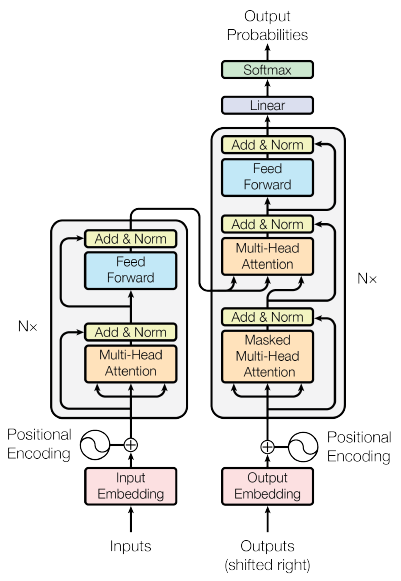
\includegraphics[width=0.5\textwidth]{figures/transformer_architecture.png}
	\caption{Transformer Architecture}
	\label{fig:transformer}
\end{figure}

\subsection{Evolution of Language Models}
It has always been difficult to teach a computer to really understand natural language. While they are capable of processing and storing large amounts of data, they lack language context. This problem continued until NLP became popular in the Artificial Intelligence field. NLP enables computers to read, analyze, interpret and gather information from long texts and single written words. In contrast to before without NLP, meaning and sense of texts can now be determined. In the beginning, a separate model was developed and used for each of these tasks. Since the development of BERT in 2018, this has changed. Engineers are now able to use a single model to handle the most common NLP tasks such as Classification, Sentiment Analysis or Question Answering. The timeline depicted in Figure \ref{fig:timeline} shows the evolution of NLP models from \alert{Bag OF Words} until \alert{BERT}.

\begin{figure}[H]
	\centering
	\includegraphics[width=1\textwidth]{figures/timeline_NLP.PNG}
	\caption{Timeline of Model evolution in NLP.}
	\label{fig:timeline}
\end{figure}

The following sections will briefly describe all of the mentioned models to cover all the important topics which will be discussed in this paper and to prepare for the technical details of BERT.

\subsection{BERT} \label{bert}
BERT  stands  for  Bidirectional Encoder Representations from Transformers. It makes use of a transformer and an attention mechanism that learns contextual relations between words or sub-words in a text. The BERT model was developed by Google researchers in 2018 and is already pre-trained using a combination of masked language modeling objective and next sentence prediction on a large corpus. The original BERT model comes in two sizes: BERT-base (trained on BooksCorpus: ~800 million words) and BERT-large (trained on English Wikipedia: ~ 2,500 million words). 
In contrast to previous language models which looked at a text sequence either from left to right or combined left-to-right and right-to-left training, BERT is using the bidirectional approach. The paper’s results show that a language model which is bidirectionally trained can have a deeper sense of language context and flow than single-direction language models. To do this, the authors introduced a new technique which is called Masked Language Modelling (MLM). \alert{This objective randomly masks 15\% tokens from an input sequence and trains on the model to predict the original vocabulary id of the masked word based on it context. This approach allows the representations to fuse context from either ends. Rather than always masking the chosen word, it masks the word 80\% times with [MASK] token, 10\% times with any random word and remaining 10\% times with the actual word, thereby biasing the prediction towards the actual observed word. Another pre-training feature introduced in BERT is ‘Next Sentence Prediction’ that takes in a sentence-pair input, replaces the second input sentence with a random sentence for 50\% of the training steps, and trains on the sentence pairs to learn sentence relationships which is needed for many downstream tasks like Question Answering and Natural Language Inference.} \newline
A Transformer usually includes two separate mechanisms, an encoder that reads the text input and a decoder that produces a prediction for the task. For producing a language model, only the encoder mechanism is necessary. Previous models have read the text input sequentially either left-to-right or right-to-left. BERT's transformer encoder reads the entire sequence of words at once. This allows the model to learn the context of a word based on all of its surroundings\alert{ \cite{Devlin}}.  \newline
The input to BERT's encoder is a sequence of tokens previously converted into vectors. Later, these tokens can be processed in the neural network. In order to be able to do this, a few steps must first be carried out:
\begin{enumerate}
	\item CLS and SEP tokens at the beginning and end of each sentence
	\item Segment embeddings for each token to distinguish between sentences.
	\item Position embeddings for each token to identify the position in a sentence.
\end{enumerate}
These three steps are depicted in Figure \ref{fig:bert_tokenizing}.

\begin{figure}[H]
	\centering
	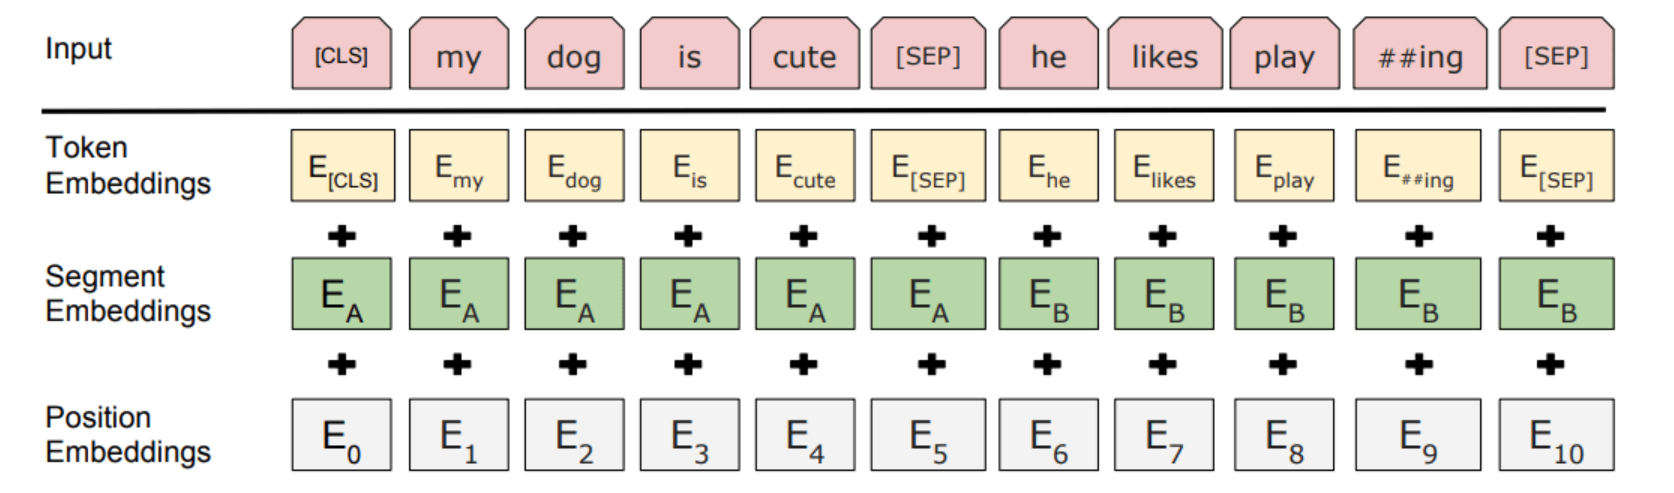
\includegraphics[width=1\textwidth]{figures/bert_tokenizing.png}
	\caption{Embeddings of Text Input with BERT.}
	\label{fig:bert_tokenizing}
\end{figure}

\begin{figure}[H]
	\centering
	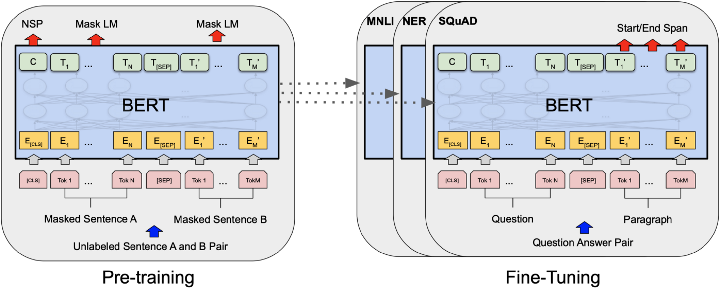
\includegraphics[width=1\textwidth]{figures/bert_training.png}
	\caption{Pre-Training and Fine-Tuning Process of BERT}
	\label{fig:bert_tokenizing}
\end{figure}

\subsubsection{Difference from BERT and word2Vec}
Word2Vec is contex-independent, so it only has a numeric vector to represent a word. If a word has several meanings, these are combined into a vector.

BERT, on the other hand, is context-dependent and thus allows multiple numeric vectors as a representation for a word, depending on the context in which the word occurs.

An example of the difference is the word bank, which can appear in a financial context as well as in a beach or park context. Word2Vec will always generate the same vector for this word and can therefore lead to an inaccurate representation. BERT can distinguish the two different semantic meanings and thus also generate two different vectors.

\begin{enumerate}
	\item The next difference is that Word2Vec doesn't care about the position of words in a sentence. BERT, on the other hand, uses the position (index) of a word as input for calculating the vector.
	\item Word2Vec only needs one word as input and delivers a vector as output. BERT, on the other hand, needs an entire sentence as input because it needs the context of the sentence to calculate the vector.
	\item Word2Vec can have problems if a word is not stored in the vocabulary and no vector can be generated. BERT can also create a vector for subwords that are not stored in the vocabulary and is therefore not limited by the vocabulary.
\end{enumerate}


\chapter{Analysis} \label{chapter:analysis}
This chapter will cover the first two research questions about existing BERT models and how well they fit to the semiconductor domain. In this way we were able to find a suitable entrypoint for training our FA-BERT model.
\section{BERT based Language Models}

\section{Finding the Model Entrypoint}
Since BERT models studied in this paper were trained on different text corpora, their tokenizers might provide different coverage of important terms used in the FA domain, such as the ones stored in FA ontology. To determine the coverage, we first analyze the tokenization of the ontology keywords with the three language models: traditional BERT, SciBERT and S2ORC-SciBERT. With this analysis it was possible to gain a first impression about the vocabulary of the models and how well they fit to the electrical domain. \newline
The models got downloaded from the website \alert{Huggingface} and can be load into the notebook as follows:
\begin{minted}{python}
	model = BertModel.from_pretrained("/path/to/model/")
	tokenizer = BertTokenizer(vocab_file = '../path/to/tokeizer/vocab.txt')
\end{minted}

To receive the keywords, we executed an existing function provided from our supervisor Christian Burmer. It executes a script with a request to the SparQL Database receiving the ontology keywords in a list. This keywords also occur in the reports as indicators for the content. \newline
After receiving the keywords from the ontology and having a deeper look at them, we found some misspellings like in the word \textit{flasover}, which misses a h to become \textit{flashover}. These typos could confuse the models and lead to some mistokenization. To prevent this, we will first run some spell checking and correction methods on the keywords before further processing it. Therefore we tried different packages like the \textit{Pyspellchecker} or \textit{SymSpellPy} which are based on the \textit\alert{{Peter Novig's method}}. As both of the two packages did not work, we skimmed the keywords manually and corrected misspellings. \newline
With the correct spelled keywords we started the experiment of tokenizing them with the three different BERT models. The code for tokenization was the same for every model:
\begin{minted}{python}
	# Run tokenizer.
	tokenized_word = s2orc_scibert_tokenizer.tokenize(word)
	
	#differentiate good and badly tokenized words
	if len(tokenized_word) == 2:
		good_tokenized_words_s2orc += 1
		good_words.extend(tokenized_word) 
	elif len(tokenized_word_c) > 2:
		badly_tokenized_words_s2orc += 1
		bad_words.extend(tokenized_word)
\end{minted}

We created a loop which hands every word over to the tokenizers and also analyzes if the resulting word is included in the models vocabulary or not. A word which is already in the vocabulary will not be divided into subtokens and so consists of only one token. If it is not included in the vocabulary, we determined if the word was good or badly tokenized. A word got considered as badly tokenized if it was split in more than two tokens. Otherwise the tokenization got considered as good. At the end of the execution, we created a dataframe depicting how the individual words got splitted into tokens. An example of the dataframe is depicted in Figure \ref{fig:goodAndBad}. Here the keyword "lifted clip" would get considered as badly tokenized word and the keyword "requestor" as good.

\begin{figure}[H]
	\centering
	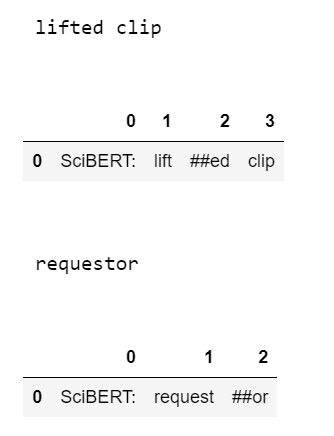
\includegraphics[width=0.3\textwidth]{figures/example_good_bad.PNG}
	\caption{Example of tokenization with SciBERT}
	\label{fig:goodAndBad}
\end{figure}


Next we analyzed the word stems of the failure analysis reports and again examined the tokenization of the words with the language models. We did not analyze the word stems of the whole reports, but only the word stems of the most frequently used words. To obtain the frequency distribution and the word stems of the reports, we used the NLTK (Natural Language Toolkit) library. It includes the so called \textit{SnowballStemmer}, because according to the documentation, this stemmer works better for English text. Stemmers remove morphological affixes from words, leaving only the word stem. To run the tokenization experiment, we also had to lower case the word stems and transform plural words into singles. The code can be seen in the code below. For the tokenization itself, the same code has been used as already explained above.

\begin{minted}{python}
	#create a new stemmer
	stemmer = SnowballStemmer("english")
	
	#test the stammer on pluralized words
	most_common_stems = nltk.word_tokenize(str(most_common))
	singles = [stemmer.stem(plural) for plural in most_common_stems]
	word_stems = set(singles)
	print(' '.join(singles))
\end{minted}

As a result of the tokenization of the keywords it can be seen that SciBERT and S2ORC-SciBERt both perform better on the keywords as the traditional BERT model. Both models contain a few more keywords in their vocabulary than the BERT model. The resulting statistic can be seen in Figure \ref{fig:comparison}. We expected this result because the training data of these two models fits better to our electrical domain than the data BERT was trained with which is more widespread.


\begin{figure}[H]
	\centering
	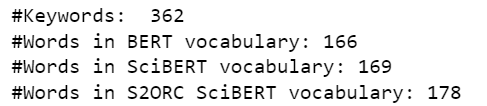
\includegraphics[width=0.5\textwidth]{figures/keyword_comparison.PNG}
	\caption{Comparison of the performance of the three models on the keywords}
	\label{fig:comparison}
\end{figure}


For the tokenization of the FA reports and their word stems we assumed to see at least a slight difference between SciBERT and S2ORC-SciBERT but without fine-tuning the models it is not possible to determine a better model which can be seen on the results of the tokenization analysis in Figure \ref{fig:stemming_performance}.


\begin{figure}[H]
	\centering
	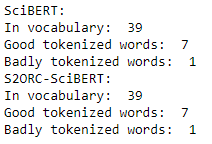
\includegraphics[width=0.3\textwidth]{figures/wordstems_comparison.PNG}
	\caption{Comparison of the performance on the word stems}
	\label{fig:stemming_performance}
\end{figure}

\alert{In order to finally decide between SciBERT and S2ORC-SciBERT, a further analysis was performed in which the keywords were assigned a weighting based on their occurrence frequency. This makes it possible to assign an importance to the keywords. The more often they appear in the reports, the more important it is that the model tokenizes the keywords well. Therefore, using the frequency and the number of subtokens, a weight is calculated as follows:}
\begin{align}
	n &= |t_1, t_2, ... t_n| \\
	\to w &= n \cdot sx_m
\end{align}

The resulting weights looked like the following:
\begin{minted}{python}
	[('thin', 0.002654), ('backside', 0.062375), ('metallization', 0.12209),...]
\end{minted}

After this weighting we again performed a tokenization and examined the good and badly tokenized keywords, but both models performed again very similar. SciBERT tokenized 129 keywords good, S2ORC-SciBERT 120. Because the FA reports contain out of more than only keywords, we decided to choose the S2ORC-SciBERT as an entrypoint for our further experiments. It has more electrical and physical papers in its training corpus than the original SciBERT and therefore might work better for us.
\chapter{Data Collection} \label{chapter:datacollection}
In order to train a language model, a sufficiently large amount of data is needed. Since the model presented in this paper will be used for textual classification, the data must be available in written form.
Most of the data used for the report classification come from the FA laboratory. The laboratory has two sources to save information: an ontology which is the formalization of FA knowledge in a computer-friendly format, and the FA reports which comprise information that describes all diagnostic steps, results, and observations for a job analysis. These two resources would have a large enough amount of data to train the model. However, experiments with previous models indicated that these documents are too specific to serve as the sole data source for a model in the semiconductor domain. The content of the documents in the ontology and the FA reports contains too specific vocabulary and too little general vocabulary about electronics and semiconductors. Models which were trained only with this data did not have sufficient performance. For this reason, additional sources were sought to train the model more extensively.
This chapter starts by introducing the inddividual datasets and how they got collected before covering the data cleaning process to prepare it as an input for the PikaBERT model. 

\section{Data Sources}
The remaining dataset was created out of different data sources which got categorized in four datasets for an easier use in later experiments. The four datasets are: the \textit{FA ontology and reports}, the \textit{S2ORC Dataset}, the \textit{Infineon Dataset} and the \textit{Additional Dataset}. The following chapters introduce every dataset with its content, size and chatateristics.

\subsection{Failure Analysis Ontology and Reports}
\alert{The  FA  laboratory  stores  most  of  its  knowledge  as  free  texts, thus they might be ambiguous and cannot be processed by the software automatically. To avoid these issues, standard definitions of FA concepts used in the domain are required.  Moreover,  these  definitions  must  be stored  in  a  way that  they  can  be  used  by  both  engineers  and software tools alike. One  possible  solution  to  this  challenge  is  to  formalize  the knowledge about the FA domain as an ontology, a knowledge base  specifically  designed  to  store  terminological  definitions. This is the case for the FA laboratory, where an ontology is being  developed,  currently  storing  hundreds  of  failures,  tasks, tools, etc. The structure of an ontology includes classes, instances of these classes  and  properties.  Individuals  are  descriptions  of  real-world entities, like sample integrated circuits of a job or tools available  in  a  lab.  Classes  are  defining  parts  of  the  world  by summarizing  properties  of  a  collection  of  individuals.}

\alert{For training the classification models, we have considered the historical  data  of  the FA  laboratory.  These  reports  contain  a series  of  fields,  including  the  job  identification  number,  cus-tomer comment regarding the issues found in devices, an anal-ysis report describing applied methods, found physical defects, their  locations,  electrical  characterization,  and  other  details. Some of this data is structured and can be retrieved from corre-sponding databases. However, the essential parts relevant to the fault  identification  process  are  described  only  in  textual  form and, therefore, cannot be processed automatically.
Consider three samples taken from fault analysis reports of an FA  Laboratory  presented  in Error!  Reference  source  not found..  The  examples  show  selected  sentences  describing  the findings  of  an  engineer  and  the  labels  indicating  the  physical faults  and  their  electrical  signatures.  Both  types  of  labels  are organized in an ontology, which is a hierarchical structure rep-resenting a taxonomy of faults. This ontology allows for the de-velopment of software tools helping to label reports manually and working with the classification results. Along  with  the  job  summary,  the  reports  contain  a  series  of fields including, an identification number of the device, lists of tasks performed on the device, the images obtained by certain tools such as X-Ray,the  description of such images attached, etc. A subset of the reports also includesfault labels, both of the electrical signature of the faulty device and of the final physical failure.For the classification phase, these two faults are considered the target  output  while  the  job  summary  and  image  descriptions will constitute the input.}

\subsection{S2ORC Dataset} \label{s2orc_dataset}
The S2ORC Dataset was collected by the Allen Institute of Artificial  Intelligence  and  it  has  a  corpus  of 81.1M  English-language academic papers from different domains. The texts  got  extracted  from  PDFs  including  abstracts  and  inline mentions of citations. The selection of subject areas is extensive and ranges from medicine and biology to geography as depicted in Figure \ref{fig:domains}.

\begin{figure}[H]
	\centering
	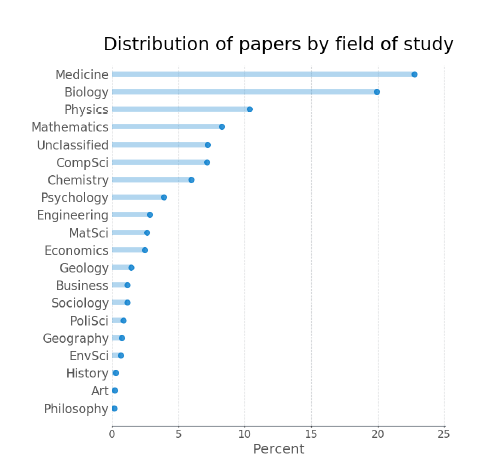
\includegraphics[width=0.6\textwidth]{figures/S2ORC_Domains.PNG}
	\caption{Different Domains in the S2ORC Dataset.}
	\label{fig:domains}
\end{figure}

Around 40\% of the papers belong to the  biomedical field, which is counterproductive for training a model in semiconductor domain. The vocabulary in the medical field partly overlaps with that in electronics, but has different meanings. A good example of this are the words neuron and electron, which are used in medicine in the field of neurology and whose semantics are related to the human brain. In electronics, this means negatively or neutrally charged particles and is related to current and voltage. For this reason, we decided to shrink the S2ORC data set and filter out only those papers that fit together in the subject area with electronics and semiconductor.
\alert{https://paperswithcode.com/paper/gorc-a-large-contextual-citation-graph-of}

\begin{figure}[H]
	\centering
	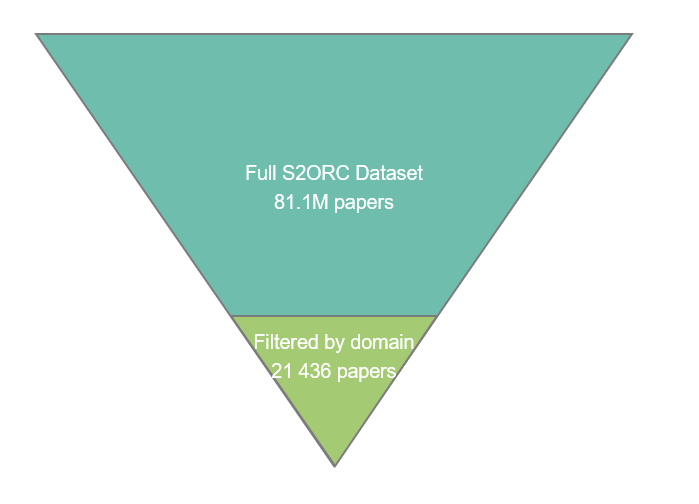
\includegraphics[width=0.6\textwidth]{figures/s2orc_filtered.PNG}
	\caption{Filtering of Domains in the S2ORC Dataset.}
	\label{fig:filtered_domains}
\end{figure}

We decided to use the following domains:
\begin{itemize}
	\item Physics
	\item Computer Science
	\item Chemistry
	\item Mathematical Science
	\item Engineering
\end{itemize}

As the selected domains form the minority of the s2orc datset, it shrank together from 81.1 Million papers to a size of about 21.000 papers as visible in Figure \ref{fig:filtered_domains}.

\subsection{Infineon Dataset}
In addition, we created an Infineon Dataset comprising rele-vant textual data available on the company’s intranet. This dataset comprises 1.687 papers covering research topics and best-practices methods in the semiconductor domain. It was collected by employees and engineers of Infineon . Be-cause these papers got collected from engineers in different countries, we had to filter out non-English language papers. After filtering and extracting the raw text, we used approxi-mately 31.5MB of text data to create a dataset.

\subsection{Additional Data}
To increase the specificity of the training data for the FA domain, we also searched the Web for FA and electrical en-gineering papers. In this work we were using open search engines, like FreeFullPDF  and GoogleScholar , as well as specific sources, like IEEE, to collect the data. The text was extracted from the papers and converted into a text represen-tation. The resulting dataset comprises 12.31MB of raw text, where 2.33MB got collected from FreeFullPDF and Google-Scholar and the other 9.98MB from IEEE.



After finishing collecting papers we ended with four independent in domain datasets collected from four different sources. We decided to unite the two smallest datasets when using it for training, what will be covered in the following chapters.
\begin{figure}[H]
	\centering
	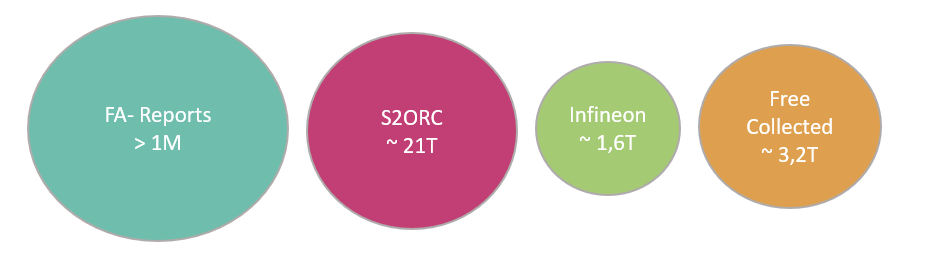
\includegraphics[width=1\textwidth]{figures/datasets.PNG}
	\caption{Overview of all collected datasets.}
	\label{fig:datasets}
\end{figure}

\section{Data Preprocessing}
For later usage during training, we combined the Infineon and the Additional Datasets in one. Moreover, since the biggest part of the S2ORC Dataset was medical and biomedical data, we filtered this dataset by using the FA ontology keywords, retaining only documents that comprise at least one keyword. The resulting filtered dataset contains approximately 542MB of raw text. For later discussions, we introduce the following abbreviations for the datasets:

\begin{itemize}
	\item \textbf{inf}: Infineon Dataset + Additional Dataset;
	\item \textbf{s2}: a part of the documents from S2ORC dataset fil-tered on keywords extracted from the ontology.
\end{itemize}

After finishing collecting the papers for the dataset, it was necessary to extract the raw text out of the documents. Therefore we got access to an text extractor API developed by Infineon collegues in Bangalore. The raw texts got extracted and UTF8 converted to be saved as excel sheets. \newline
Not all of the extracted text is important or useful for the dataset. To remove unuseful data, a notebook was created were the text got prepared before being cleaned. Authors, metadata about the images, tables and other not contiguous text was remoed. The resulting text got again saved as excel sheets.

\subsection{Data Cleaning}
To use the FA reports for AI purposes, their content must be pre-processed and cleaned to erase all data that can disrupt the training process. One of the biggest issues regarding the FA reports is the wide variety of styles in which they are written, as they come from several laboratories around the globe, some of them dealing with specific purposes, while others deal with a broader range of failures. It is also essential to consider that although all they are written in English, this is not a standard language as engineers are only rarely native speakers. \newline
The data cleaning process was the same for all datasets. A notebook was created were the excel sheets got loaded into dataframes. The methods used for cleaning the text are imported from the \alert{Natural Language Toolkit (nltk)} package which implements functions for normalization, stemming and lemmatization.
The following steps describe the procedure of text cleaning:

\begin{enumerate}
	\item \textbf{Remove Punctuations and Special Characters}: Punctuatins and special characters got removed inbetween and at the end of every sentence by using regular expressions because a language model is not able to interpret those characters. 
	\item \textbf{Remove Numbers}: The input got checked if it is a number or not. Also all words which are not strictly all letters got removed to avoid confusing the model.
	\item \textbf{Normalization}: After removing undesired words and characters, the entire text got normalized. This means that the resulting text contains only out of lowercased letters.
	\item \textbf{Remove Stop-Words}: The nltk package contains a collection of english stop-words like "and", "or", "but", "for" etc. Due to their low entropy they are useless for the training and therefore removed from the text.
	\item \textbf{Lemmatization}: Lemmatization considers the context of a word and converts it to its meaningful base form, which is called Lemma. For instance, lemmatizing the word "Caring" would return "Care". This has been done for the entire dataframe by iterating over the words.
	\item \textbf{Remove Empty Lines}: Due to the previous cleaning some cells or lines of the dataframe may be empty now and represented as NaN values in the dataframe. These NaN values have to be replaced with spaces, otherwise they will cause errors during further processing.
\end{enumerate}


\subsection{Dataset Formatting}
In comparison to traditional neural networks, BERT-based models are like a black box for the engineer. For training the model we used the so-called “transformer” class from \alert{Huggingface}.  The trainer method of the transformer class needs a model, a tokenizer and the training dataset as input. This input dataset needs to have a specific format and datatype otherwise the function would rise an error.  To do so the previous created dataframes got converted into dataframes of two cells, an index and a text cell. An example is shown in Table \ref{tab:format}.

\begin{table}[H]
	\centering
	\begin{tabular}{ll}
		\hline
		& \textbf{text}                                         \\ \hline
		0 & The following parameters are most often considered... \\ \hline
		1 & Nitrogen fertilization stands out as an important...  \\ \hline
	\end{tabular}
	\caption{Example of transformed dataframe shape}
	\label{tab:format}
\end{table}

The base class \textit{Dataset} from Huggingface implements a Dataset backed by an Apache Arrow table. This type of object can be created out of the dataframe just created with the following code:

\begin{minted}{python}
		train_dataset = Dataset.from_dict(df)
		datasets = datasets.DatasetDict({"train:" train_dataset})
\end{minted}

The dataset object allows to specify a training and a test dataset. Since training the language model is an unsupervised learning method, only the training dataset is needed. The resulting dataset objects were saved and could be loaded later for training.

\alert{Tokenizing dataset
split into blocks}
\chapter{Experiments} \label{chapter:experiments}
In this section we will cover the process of preparing the collected dataset, described in section \ref{chapter:datacollection} and training different types of tokenizers and language models until we found the best performing one.

\section{Tokenization of the dataset}
In order to use the dataset created earlier in the chapter \ref{chapter:datacollection} for the BERT based model as training input, it must be transformed into a suitable format. Since we are using the Huggingface trainer, we also need to follow the Huggingface training data format. \newline
In the first step, the entire text from the CSV file is converted into a dataset dictionary. This is possible with one line of code after importing the datasets package.

\begin{code}
\captionof{listing}{Creating the Dataset Dictionary}
\label{code:dict}
\begin{minted}{python}
from datasets import Dataset
training_data = Dataset.from_dict(df)
datasets = datasets.DatasetDict({"train": train_data})
	\end{minted}
\end{code}

When using this method, training and test data can be stored together in one object and accessed via the datasets["train"] or datasets["test"] index. The resulting datasets["train"] dictionary has the feature "text" to access the data and 1.052.587 rows as visible in the output depicted in Figure \ref{fig:dict_features}.
\begin{figure}[H]
	\centering
	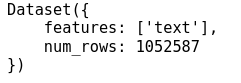
\includegraphics[width=0.4\textwidth]{figures/dataset_dict_features.png}
	\caption{Format of Dataset Dictionary}
	\label{fig:dict_features}
\end{figure}

The next step is to apply the tokenizer to the entire text. For this we use the map method from the datasets library. First we define a method shown in Listing \ref{code:tok_funct} which calls the tokenizer on the text.

\begin{code}
	\captionof{listing}{Tokenize Function to call on the text}
	\label{code:tok_funct}
	\begin{minted}{python}
def tokenize_function(examples):
return tokenizer(examples["text"])
	\end{minted}
\end{code}

The map function, shown in Listing \ref{code:tok_map}, can be used to apply the tokenizer function from Listing \ref{code:tok_funct} to the entire dataset. To speed up the process, we pass the number\_poc=4 attribute, which enables multithreading and splits the process into four threads.

\begin{code}
	\captionof{listing}{Applying the tokenize function on the Text}
	\label{code:tok_map}
	\begin{minted}{python}
tokenized_datasets = datasets.map(tokenize_function, batched=True, num_proc=4, 
	remove_columns=["text"])
	\end{minted}
\end{code}

The "text" collumn from the dictionary has now been replaced by the input\_ids which is needed by the modell as an input for training.

\begin{figure}[H]
	\centering
	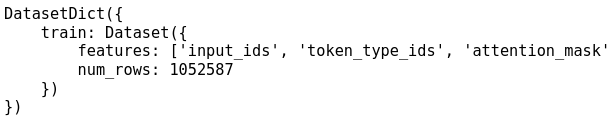
\includegraphics[width=0.8\textwidth]{figures/tok_dataset.png}
	\caption{Text collumn has been replaced by calling tokenizer on the dataset.}
	\label{fig:dict_tokenized}
\end{figure}

After the dataset has been tokenized, the next step is to split it into individual chunks. The size of these chunks depends on the available resources and the maximum context size of the model. The context size can be determined with the method \alert{model\_max\_length}. For BERT based models, like ours, it is 512 tokens.
We need to concatenate all of our texts together and then split the result in small chunks of a certain \alert{chunk\_size}. To do this, we will use the \alert{map} method again, with the option \alert{batched=True}. This option actually lets us change the number of examples in the datasets by returning a different number of examples than we got. This way, we can create our new samples from a batch of examples.\newline
First, we grab the maximum length our model was pretrained with. This might be a big too big to fit in our GPU RAM. In the first try we chose a chunk size of 64, which turned out not to be suitable because longer sentences were truncated, while shorter sentences were populated with [PAD] tokens (id: 0) until they reach the desired length. Using a small chunk size can be detrimental in real-world scenarios, so it is recommended to use a size that corresponds to the use case the model will be applied to. Because of that we chose a chunk size of 128.

\begin{code}
	\captionof{listing}{Definition of the method group\_text}
	\label{code:group_text}
	\begin{minted}{python}
chunk_size = 128

def group_texts(examples):
# Concatenate all texts
concatenated_examples = {k: sum(examples[k], []) for k in examples.keys()}
# Compute length of concatenated texts
total_length = len(concatenated_examples[list(examples.keys())[0]])
# We drop the last chunk if it's smaller than chunk_size
total_length = (total_length // chunk_size) * chunk_size
# Split by chunks of max_len
result = {
	k: [t[i : i + chunk_size] for i in range(0, total_length, chunk_size)]
	for k, t in concatenated_examples.items()
}
# Create a new labels column
result["labels"] = result["input_ids"].copy()
return result
	\end{minted}
\end{code}


\section{Training of the Tokenizer}\label{sec:tokenizer}
Also the tokenizer itself can be improved before using it in the training method together with the model. Training a tokenizer can be done in two ways:

\begin{enumerate}
	\item Extending the vocabulary manually
	\item Pre-training the tokenizer 
\end{enumerate}

Tokenizers of BERT-derived models usually have empty positions allowing us to add required tokens directly. Extend-ing the vocabulary of a tokenizer means that it won’t get trained explicitely but important words like our ontology keywords can be added to the vocabulary of the tokenizer and therefore recognized as one single token by the model later. Pre-training the tokenizer means that the tokenizer will get trained on a prepared dataset without using the model. Again the engineer has no impact on the behavior of the tokenizer during the training loops. 
We created four types of trained tokenizers. For later discussions we introduce the following abbreviations:

\begin{itemize}
	\item \textbf{ext}: A tokenizer with the ontology keywords added to its vocabulary manually
	\item \textbf{small}: A tokenizer trained on inf dataset
	\item \textbf{large}: A tokenizer trained on inf+s2 dataset;
	\item \textbf{flt}: A tokenizer trained on the s2 dataset
\end{itemize}

\subsection{Extending the tokenizers vocabulary}
For the first experiment we tried to enhance the language models performance by extending the tokenizers vocabulary. The tokens which we added to the vocabulary were the ontology keywords. As already discussed in the \alert{section before}, some of the keywords included misspellings. We again removed or corrected these keywords to avoid to sabotage our model. \newline
Before extending the tokenizer, it's vocabulary had a size of 31944. To add the keywords to he tokenizers vocabulary, we had to execute the following code:

\begin{code}
	\captionof{listing}{Extending the Tokenizer Vocabulary}
	\label{code:extend_tokenizer}
\begin{minted}{python}
	for keyword in keywords:
		tokenizer.add_tokens(keyword)
\end{minted}
\end{code}

The keywords got added to the vocabulary and increased the vocabulary size to 32131. After saving the tokenizer it can be used in the training process like any other pretrained tokenizer.

\subsection{Pre-Training the tokenizer}\label{chapter:training-tokenizer}
Training a tokenizer is very simple with the\alert{ huggingface} methods. To train a tokenizer we first need to create a training dataset again. This dataset should have the same format as already discribed in chapter \ref{chapter:datacollection}. For our experiments, we assembled four different datasets to train four tokenizers. These were then to be trained together with the language model in different tests. The different data sets were used for testing purposes to find the best possible model.

\alert{creating of the training corpus}


After creating the training corpus, the tokenizer can be trained with one single line of code. The \alert{train new from iterator} method needs the training corpus and the new vocabulary size as an input. We chose the highest possible vocabulary size, which is 52.000.

\begin{code}
	\captionof{listing}{Training the Tokenizer and resize Vocabulary}
	\label{code:train_tokenizer}
\begin{minted}{python}
	tokenizer = old_tokenizer.train_new_from_iterator(training_corpus, 52000)
\end{minted}
\end{code}
After training the tokenizer with the smaller training corpus, it tokenized the ontology keywords into 542 tokens instead of 661, which means an improvement in performance.

\section{Training Process}
\alert{The training process for all of the following experiments is the same and will be discribed below.}
After creating the training data as described in section \ref{chapter:datachunking}, it is necessary to prepare some requirements for the training process. The whole training is executed on the HPC Cluster, \alert{described in section \ref{chapter:hpc}}, \alert{to ensure the training can be executed as fast as possible}.
\alert{Most of the training code got copied from the huggingface notebook. The relevant code is described in the section Masked Language Modeling}. It also includes the process of how to chunk the training dataset into a specific block size which is needed by the model as an input. We adapted the code regarding to our needings. \newline
The training itself contains out of the five steps:
\begin{enumerate}
	\item Defining the model and tokenizer checkpoints
	\item Chunking the dataset into blocks
	\item Defining the training arguments
	\item Defining the Huggingface Trainer
	\item Call the train method
\end{enumerate}

Defining the model and tokenizer checkpoints can be done in the same way as shown in the code \ref{code:checkpoint}. The chunking of the dataset is described in section \ref{chapter:datachunking}. The training arguments are variables which are needed by the trainer object. Here different values like the learning rate, the name of the model and how to report the logging can be set.

\begin{code}
	\captionof{listing}{Creating the Training Arguments}
	\label{code:train_args}
\begin{minted}{python}
training_args = TrainingArguments(
"checkpoint_LM_s2_s2orc",
evaluation_strategy = "epoch",
learning_rate=2e-5,
weight_decay=0.01,
report_to="tensorboard,
logging_strategy="steps"
)
\end{minted}
\end{code}

\begin{code}
	\captionof{listing}{Creating the Trainer Object}
	\label{code:trainer}
\begin{minted}{python}
trainer = Trainer(
model=model,
args=training_args,
train_dataset=lm_datasets["train"],
data_collator=data_collator,
)
\end{minted}
\end{code}

The training can be started by calling the method train() from the \alert{transformers trainer object.}
\begin{code}
	\captionof{listing}{Starting the training}
	\label{code:train}
\begin{minted}{python}
trainer.train()
\end{minted}
\end{code}

\subsection{Moving the bias towards FA domain}\label{chapter:training-experiments}
In the first training experiments it was our goal to move the bias of the pretrained S2ORC-SciBERT further towards the semiconductor and failure analysis domain. Therefore we use different datasets. 

\alert{discribe datasets here}

For later discussions and easier use we introduce the following abbreviations:
\begin{itemize}
	\item \textbf{inf}: Infineon Dataset (FA-reports, FA-papers, IEEE papers, FreeFullPDF papers)
	\item \textbf{s2}: S2ORC dataset filtered on keywords
\end{itemize}

For the first few experiments we used the inf dataset together with the different trained and extended tokenizers explained in section \ref{sec:tokenizer}. The inf dataset should be a good complement to the BERT based model which has already been pre-trained with the S2ORC dataset. With the help of the trained tokenizers, this training material should prepare for the classification of FA reports. We trained the models for 10 epochs and a learning rate of 2e-5 as described in Listing \ref{code:trainer}. In the descriptions of the following experiments we refer to the abbreviations described in section \ref{chapter:training-tokenizer} and section \ref{chapter:training-experiments}. \newline

\textbf{Experiment 1:}\\
For the first experiment we trained the S2ORC-SciBERT with the \textit{inf} dataset and used the pre-trained tokenizer \textit{small} for 10 epochs. We started with a loss of about 8. The loss curve falls steadily. A small hill can be seen in the area around 40k steps. This indicates that the model was not training optimally at this point and had to adjust its weights. After 10 epochs the loss reached a value of 3.471.
\begin{figure}[H]
	\centering
	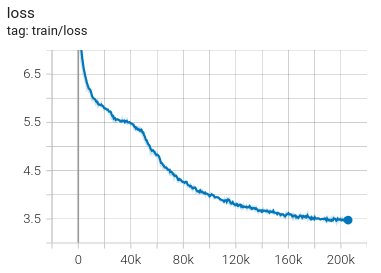
\includegraphics[width=0.6\textwidth]{figures/loss_inf_small.png}
	\caption{Loss Function during Training with Infineon Dataset and small trained tokenizer.}
	\label{fig:loss_small}
\end{figure}

\textbf{Experiment 2:}\\
In the second experiment we used the \textit{inf} dataset again together with the pre-trained tokenizer \textit{large} for 10 epochs. We started with a loss of about 8.5. The loss curve falls steeper at the beginning before it flattens out. Although the training seemed promising, int the end the loss reached again a value of 3.471 after 10 epochs.
\begin{figure}[H]
	\centering
	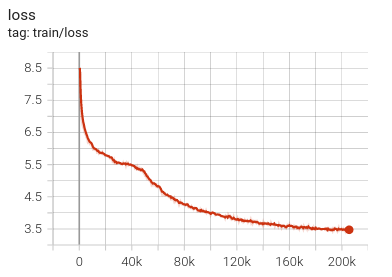
\includegraphics[width=0.6\textwidth]{figures/loss_inf_large.png}
	\caption{Loss Function during Training with Infineon Dataset and large trained tokenizer.}
	\label{fig:loss_large}
\end{figure}

\textbf{Experiment 3:}\\
To compare a pre-trained tokenizer with the extended tokenizer approach, we used the \textit{ext} tokenizer together with the \text{inf} dataset in experiment three. The loss curve behaves similarly to that of experiment two. In the end it flattens out at a loss value of 3.475, which is slightly higher than in experiment one and two.
\begin{figure}[H]
	\centering
	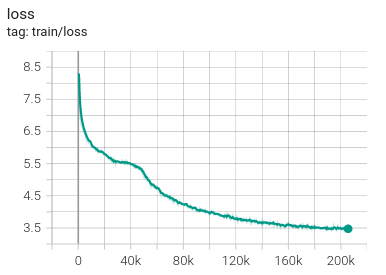
\includegraphics[width=0.6\textwidth]{figures/loss_inf_ext.png}
	\caption{Loss Function during Training with Infineon Dataset and extended tokenizer.}
	\label{fig:loss_ext}
\end{figure}

\textbf{Experiment 4:}\\
For experiment four we went for a bigger dataset, \textit{inf} dataset combined with \textit{s2} dataset, and trained it together with the tokenizer \text{flt} which is the one with the largest vocabulary. Surprisingly, the loss curve hardly changes at all and flattens out at a loss value of again 3.471 after 10 epochs.
\begin{figure}[H]
	\centering
	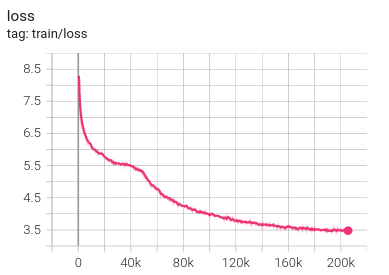
\includegraphics[width=0.6\textwidth]{figures/loss_infs2_s2.png}
	\caption{Loss Function during Training with tokenizer trained on s2.}
	\label{fig:loss_s2}
\end{figure}

\textbf{Experiment 5:}\\
As for the last experiments the loss curve hardly changed, we decided to increase the number of training epochs to 15. We sticked with the combination fo the datasets \textit{inf} and \textit{s2} and used the tokenizer \textit{large} as it showed the steepest loss curve at the beginning. The additional 5 epochs showed an improvement compared to the previous training sessions, the loss courve flattens out at a value of 3.088.
\alert{Bild später ersetzen}
\begin{figure}[H]
	\centering
	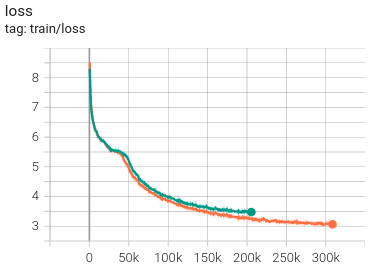
\includegraphics[width=0.6\textwidth]{figures/loss_infs2_large.png}
	\caption{Loss Function during Training with largest dataset and tokenizer trained on large.}
	\label{fig:loss_large_large}
\end{figure}

\alert{Hier Bild von gemeinsamen kurven einfügen}

The various loss functions hardly differ from each other. On the basis of the last curve, which was trained for 15 epochs, it can be seen that the longer training could certainly lead to a better performance. Nevertheless, the loss function already flattens out too much in this area. For this reason, further \alert{ measures} regarding the improvement of the training were researched.

\subsection{Trying different types of losses}
Another attempt to improve the performance of the model is to implement a different loss function. Cross entropy loss seemed to be particularly suitable. In the case of masked language modeling, this metric compares the token predicted by the model with the ground truth and assigns a value between 0 and 1 to the prediction. 0 stands for a perfect prediction. During training, the values are aggregated to represent the loss function. \newline
The loss function used by the \alert{Trainer object from Huggingface Transformers} is shown in Listing \ref{code:loss}.

\begin{code}
	\captionof{listing}{Trainer compute loss function}
	\label{code:loss}
\begin{minted}{python}
def compute_loss(self, model, inputs, return_outputs=False):
	if self.label_smoother is not None and "labels" in inputs:
		labels = inputs.pop("labels")
	else:
	labels = None
	outputs = model(**inputs)
	# Save past state if it exists
	if self.args.past_index >= 0:
		self._past = outputs[self.args.past_index]
	
	if labels is not None:
		loss = self.label_smoother(outputs, labels)
	else:
	# We don't use .loss here since the model may return tuples 
	# instead of ModelOutput.
	loss = outputs["loss"] if isinstance(outputs, dict) else outputs[0]
	
	return (loss, outputs) if return_outputs else loss
\end{minted}
\end{code}
\alert{quelle: https://github.com/huggingface/transformers/blob/v4.17.0/src/transformers/trainer.py#L2006}

which means that, by default, the model itself is responsible for computing some sort of loss and returning it to outputs. To implement an own loss function, we had to overwrite the Trainer class and the loss function and defining a cross entropy loss function to return it to outputs. The code is shown in listing \ref{code:cel}. We use the cross entropy loss function from \alert{torch.nn} here. In most cases the \alert{CrossEntropyLoss(}) function gets some weights as inputs, but because in our case pretraining a BERt model is an unsupervised learning task, we have no weights to assign and leave it empty.

\begin{code}
	\captionof{listing}{Cross Entropy Loss}
	\label{code:cel}
\begin{minted}{python}
class MyTrainer(Trainer):
	def compute_loss(self, model, inputs, return_outputs = False):
		labels = inputs.pop("labels")
		outputs = model(**inputs)
		logits = outputs.get("logits")

		loss_fct = nn.CrossEntropyLoss()
		loss = loss_fct(logits.view(-1, tokenizer.vocab_size),
				labels.view(-1))
		return (loss, outputs) if return_outputs else loss
\end{minted}
\end{code}

\subsection{Changing the Masking Method}
The original masking method which is used by all BERT based models is that every token in an input blocked gets masked by the probability of 15\%. 
\alert{hier fehlt noch was}

Based on the latest experiments, it can be seen that our models are not sufficiently well trained in the semiconductor area. Another attempt to improve the performance is to adjust the masking strategy during the training. After some research we came across the Whole Word Masking strategy. With this method, not only some tokens are randomly masked, but it is also checked whether the token to be masked is a standalone token or a subtoken. If a subtoken, which is part of a word, should get masked, the algorithm also masks all the surrounding tokens that belong to the word. In addition we increased the masking probability from 15\% to 20\%. The code is visible in Listing \ref{code:wwm}. Therefore we created a new data collator class \alert{which has the whole word masking method implemented} and handed this data collator to the trainer shown in Listing \ref{code:trainer_wwm}.

\alert{nicht vergessen tokenizer map funktion geändert damit word ids im dataset}
\begin{figure}[H]
	\centering
	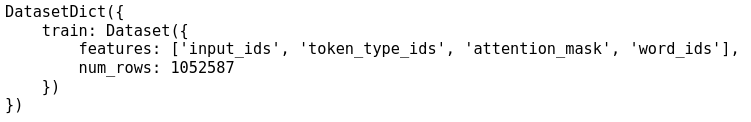
\includegraphics[width=1\textwidth]{figures/tok_dataset_wordids.png}
	\caption{Loss Function during Training with Infineon Dataset and large trained tokenizer.}
	\label{fig:data_wordids}
\end{figure}

\begin{code}
	\captionof{listing}{Data Collator implementing Whole Word Masking}
	\label{code:wwm}
\begin{minted}{python}
wwm_probability = 0.2

def whole_word_masking_data_collator(features):
	for feature in features:
	word_ids = feature.pop("word_ids")
	
	# Create a map between words and corresponding token indices
	mapping = collections.defaultdict(list)
	current_word_index = -1
	current_word = None
	for idx, word_id in enumerate(word_ids):
	if word_id is not None:
	if word_id != current_word:
	current_word = word_id
	current_word_index += 1
	mapping[current_word_index].append(idx)
	
	# Randomly mask words
	mask = np.random.binomial(1, wwm_probability, (len(mapping),))
	input_ids = feature["input_ids"]
	labels = feature["labels"]
	new_labels = [-100] * len(labels)
	for word_id in np.where(mask)[0]:
	word_id = word_id.item()
	for idx in mapping[word_id]:
	new_labels[idx] = labels[idx]
	input_ids[idx] = tokenizer.mask_token_id
	feature["labels"] = new_labels
	
	return torch_default_data_collator(features)
\end{minted}
\end{code}

\alert{Figure \ref{fig:wwm_ex} shows an example of how the whole word masking method works. The green examples shows how the algorithm is masking all surrounding subtokens which belong to a word were the blue example show some random picked tokens to mask which do not belong to any other word.}

\begin{figure}[H]
 	\centering
 	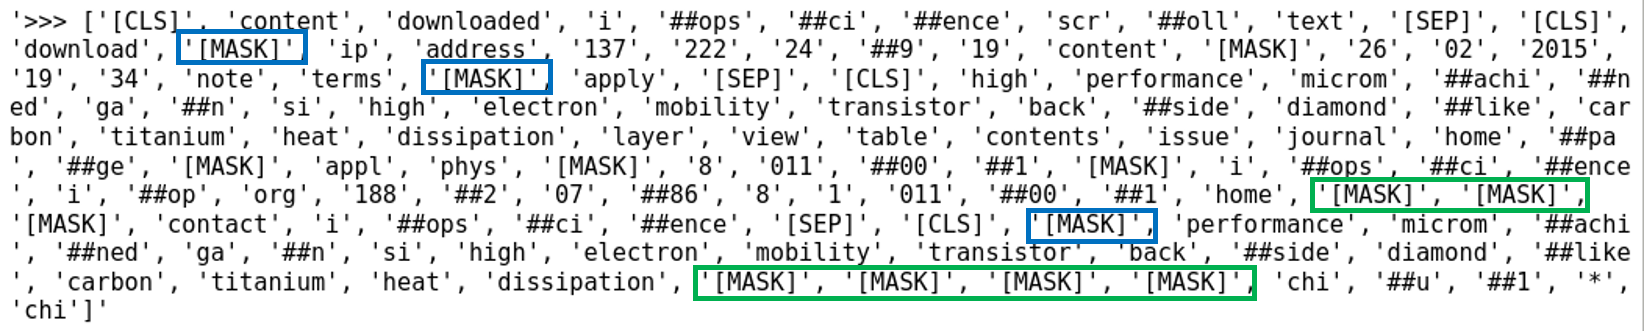
\includegraphics[width=1\textwidth]{figures/wwm_example.png}
 	\caption{Example of Whole Word Masking Method.}
 	\label{fig:wwm_ex}
 \end{figure}

\begin{code}
\captionof{listing}{Trainer}
\label{code:trainer_wwm}
\begin{minted}{python}
trainer = MyTrainer(
model=model.to(device),
args=training_args,
train_dataset=lm_datasets['train'],
data_collator=whole_word_masking_data_collator,
tokenizer=tokenizer
)
\end{minted}
\end{code}

We trained the model with the new masking method again for 20 epochs and the same learning rate and weight decay as in the other experiments. The results show a final loss of 2.51, which is the lowest loss in all experiments so far. The loss curve is depicted in Figure \ref{fig:loss_wwm}. This model could allow a good performance for the FA classifier after further training epochs. 

\begin{figure}[H]
	\centering
	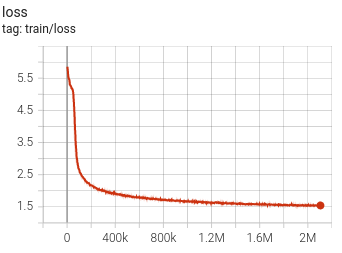
\includegraphics[width=0.6\textwidth]{figures/loss_wwm_20.png}
	\caption{Loss Function during Training with Whole Word Masking.}
	\label{fig:loss_wwm}
\end{figure}
\chapter{Results} \label{chapter:results}
\section{Performance Measures}
\section{Discussion of Results}	Inhalt...



\chapter{Conclusion} \label{chapter:conclusion}

\section{Future Work}


%%=========================================================================================================================================
%=========================================================================================================================================
\chapter{Tipps} \label{chapter:tipps}
%=========================================================================================================================================
%=========================================================================================================================================
In diesem Kapitel haben wir einige Tipps und Richtlinien zusammengestellt, die Sie Im Rahmen Ihrer Arbeit ber�cksichtigen sollten. Die
Ausf�hrungen erheben keinen Anspruch auf Vollst�ndigkeit und Richtigkeit.

%-----------------------------------------------------------------------------------------------------------------------------------------
\section{Wichtiges zum Ablauf der Masterarbeit}
%-----------------------------------------------------------------------------------------------------------------------------------------

%--------------------------------------------------------------------
\subsection{Am Anfang}
%--------------------------------------------------------------------
\begin{itemize}
  \item Literaturrecherche zum Thema (Bibliothek, Online-Ressourcen, \ldots)
  \item Nach Diskussion mit der Betreuerin bzw. dem Betreuer \\
        \ra Abgabe der Gliederung und Besprechung \\
        \ra Pr�sentation der geplanten Arbeit im Privatissimum (\qq{Was m�chte ich (wie/womit) machen?})
  \item Nach Startvortrag: elektronische Anmeldung der Masterarbeit
  \item Sie gehen auf die {\bf m�ndliche} Masterpr�fung zu. Wenn Sie bisher nur wenige m�ndliche Pr�fungen abgelegt haben, dann sollten Sie noch bei ein paar Pr�fungen �ben, damit es bei der Masterpr�fung keine Probleme gibt.
  \item H�ren Sie, wenn m�glich, bei anderen Masterpr�fungen zu. Dann sind Sie bei Ihrer Masterpr�fung nicht von der Atmosph�re
      �berrascht. Zudem k�nnen Sie so die f�r Sie passenden Pr�ferinnen  und Pr�fer leichter bestimmen.
\end{itemize}

%--------------------------------------------------------------------
\subsection{Nach dem ersten Drittel}
%--------------------------------------------------------------------
\begin{itemize}
  \item Elektronische Abgabe eines aussagekr�ftigen Probekapitels (20 Seiten Text mit Tabellen, Abbildungen und Referenzen). Hier
      kann Sie (oder besser: den Betreuenden) ein Probedruck vor b�sen �berraschungen (z.B. unleserliche Schriften, schwarze Bl�cke in
      Abbildungen) bewahren.
  \item Sie erhalten das Probekapitel nach 7-10 Tagen mit Anmerkungen zur�ck.
\end{itemize}

%--------------------------------------------------------------------
\subsection{Nach der H�lfte (oder zumindest 1  Mal pro Semester)}
%--------------------------------------------------------------------
\begin{itemize}
  \item Pr�sentation des aktuellen Standes der Arbeit (1 Teilthema vertiefen) im Privatissimum (\qq{Was mache ich gerade und wie geht's weiter?})
  \item �berpr�fen, ob alle n�tigen Zeugnisse und Bescheinigungen vorliegen, und ob der 3. Abschnitt eingereicht ist.
\end{itemize}

%--------------------------------------------------------------------
\subsection{Endphase der Masterarbeit }
%--------------------------------------------------------------------
{\textbf Tipp:} Pr�fungsbuch fr�h checken, damit es am Ende zu keinen Problemen (und damit Verz�gerungen) kommt. Zudem Pr�ferinnen bzw. Pr�fer, und Pr�fungsgebiete fr�h aussuchen und Termin koordinieren! Im Zweifel bei einer studienabschlie�enden Pr�fung (STAP -- aka Masterpr�fung) zuh�ren. Die aktuellen Termine finden Sie im virtuellen Schaukasten (siehe \url{https://campus.aau.at/antraege/public/stap}).
\begin{itemize}
  \item Endvortrag im Privatissimum (\qq{Was habe ich (wie/womit) gemacht und gelernt?})
  \item Einreichung des Pr�fungsbuches (i.d.R. 1 Woche bis zur Genehmigung)
  \item Abgabe der Masterarbeit (nur noch elektronisch, handschriftliche Unterschrift ersetzen durch \qq{$<Vorname>$ $<Nachname>$ e.h.}. Ihre Betreuerin bzw. Ihr Betreuer freut sich trotzdem �ber ein gebundenes Exemplar.
  \item Begutachtungsphase der Masterarbeit (maximal 8 Wochen)
  \item Mit Vorliegen der Genehmigung des Pr�fungsbuches und des Gutachtens kann der Antrag zur studienabschlie�enden Pr�fung elektronisch �ber das Studierendenportal (\qq{Meine Antr�ge} gestellt werden.
  \item Der Pr�fungstermin und die Pr�ferinnen bzw. Pr�fer (i.d.R. drei: Vorsitzende/r, erste/r und zweite/r Pr�fer/in) sind von Ihnen selbst zu organisieren.  Bitte beachten Sie, dass bei Antragstellung der Pr�fungstermin mindestens 3 Wochen in der Zukunft liegen muss, sonst ist eine Antragstellung nicht m�glich. Diese Frist ist in der Satzung der Alpen Adria Universit�t festgelegt. Damit ergibt sich ein maximaler Zeitraum von 11 Wochen zwischen dem Einreichen der Masterarbeit und der STAP!
  \item Die drei Pr�fungsgebiete sind in der Pr�fungsordnung Ihres Curriculums geregelt und beinhalten die Pr�sentation und Verteidigung der Masterarbeit, das Spezialisierungsgebiet und ein weiteres Fach aus den Erg�nzungs- oder Spezialisierungsf�chern.
  \item In diesem Online-Antrag k�nnen Sie Anmerkungen wie zB. Vorschl�ge f�r den Pr�fungsort oder andere Informationen hinterlassen. Sie werden nach der Genehmigung durch den Studienprogrammleiter per Mail �ber den Pr�fungstermin verst�ndigt. Sie haben �ber diesen Online-Antrag auch die M�glichkeit, bis 24 Stunden vor der Pr�fung den Antrag ohne Angabe von Gr�nden zur�ckzuziehen.
  \item Ihr Pr�fungstermin wird im Intranet der AAU im virtueller Schaukasten (siehe \url{https://campus.aau.at/antraege/public/stap}) ver�ffentlicht.
  \item Alle Ver�nderungen bei diesem Online-Antrag werden per E-Mail mitgeteilt, deshalb achten Sie auch darauf, dass der Posteingang Ihres Uni-Email-Accounts nicht �berf�llt ist, da ansonsten diese Informationen nicht zugestellt werden k�nnen!
\end{itemize}

%--------------------------------------------------------------------
\subsection{Endlich: Der Vortrag bei der Masterpr�fung (oder Endpr�sentation)}
%--------------------------------------------------------------------
\begin{itemize}
  \item Wie w�rden Sie Ihre Masterarbeit mit zwei (bis drei) S�tzen beschreiben?
  \item Worauf sind Sie besonders stolz?
  \item Kurzer �berblick, damit alle Anwesenden wissen, was Sie geleistet haben.
  \item Ein (zwei) Themen herausgreifen und vertieft erl�utern, damit Sie einerseits ``gl�nzen'' k�nnen und die Anwesenden m�glicherweise etwas Neues lernen.
\end{itemize}

%--------------------------------------------------------------------
\subsection{Diverses}
%--------------------------------------------------------------------
\begin{itemize}
  \item Unterlagen vor Abgabe in der Studienabteilung kopieren.
  \item Mit Ablegen der Masterpr�fung verlieren Sie den Status ``Studierende'' bzw. ``Studierender'' und k�nnen somit gegebenenfalls
      auf Sammelzeugnisse oder �hnliche Daten nicht mehr zugreifen. Diese Daten sollten Sie vor der Masterpr�fung
      ausdrucken bzw. als PDF speichern.
  \item Eventuell im letzten Semester ein Zweitstudium inskribieren, damit man wenigstens noch eingeschr�nkten
      Zugang auf seine Daten hat.
\end{itemize}

%-----------------------------------------------------------------------------------------------------------------------------------------
\section{Wichtiges zu Bachelorarbeiten}
%-----------------------------------------------------------------------------------------------------------------------------------------
\begin{itemize}
  \item Eine Bachelorarbeit muss vor Beginn als solche deklariert und angemeldet werden.
  \item Abstract: 170-250 W�rter
  \item Umfang: ca. 8000 W�rter (tats�chlicher Umfang obliegt den Vorgaben der Betreuerin bzw. des Betreuers)
  \item Sprache: nach R�cksprache mit der Betreuerin bzw. dem Betreuer
\end{itemize}

%-----------------------------------------------------------------------------------------------------------------------------------------
\section{Wichtiges zu Seminararbeiten}
%-----------------------------------------------------------------------------------------------------------------------------------------
\begin{itemize}
  \item Abstract: 170-250 W�rter
  \item Umfang: ca. 5000 W�rter (tats�chlicher Umfang obliegt den Vorgaben der Betreuerin bzw. des Betreuers)
  \item Sprache: nach R�cksprache mit der Betreuerin bzw. dem Betreuer
\end{itemize}

%-----------------------------------------------------------------------------------------------------------------------------------------
\section{Richtlinien und Tipps f�r wissenschaftliche Arbeiten}
%-----------------------------------------------------------------------------------------------------------------------------------------

%--------------------------------------------------------------------
\subsection{�u�ere Form}
%--------------------------------------------------------------------
\begin{itemize}
  \item Die Masterarbeit wird bei Ihren zuk�nftigen Bewerbungen ein wesentliches Kriterium sein. Der erste Eindruck, den Ihre
      Arbeit hinterl�sst wird immer ein optischer sein! Neben den inhaltlichen Aspekten sollten Sie daher auch auf das �u�ere
      Erscheinungsbild Ihrer Arbeit Wert legen.
  \item Formatierung und Daten der Titelseite und ``Eidesstattliche Erkl�rung'' laut aktuellen Vorschriften der Studienabteilung!
  \item Schrift 11pt Times New Roman, Zeilenabstand 110\%, Blocksatz mit Silbentrennung.
  \item Seitengr��e DIN-A4, R�nder r/l/o/u = 2,5/3,0/2,5/2,5 cm
  \item Doppelseitiger Druck (Kopfzeilen beachten), Kapitelbeginn auf ungerader (rechter) Seite:
        \begin{itemize}
          \item linke Seite:  \underline{Seiten-Nr \hspace*{5cm} Kapitelname}
          \item rechte Seite: \underline{Abschnittsname \hspace*{5cm} Seiten-Nr}
        \end{itemize}
  \item Umfang der Arbeit nach Vereinbarung (Qualit�t geht vor Quantit�t). Es gelten jedoch folgende Richtwerte:
        \begin{itemize}
          \item Masterarbeit:         $\pm$  100 Seiten
          \item Bakkalaureatsarbeit:  $\pm$ 8000 Worte
          \item Bericht (SWP/WFP):    $\pm$   30 Seiten
          \item Seminararbeit:        $\pm$ 5000 Worte
        \end{itemize}
  \item Sprache nach Vereinbarung -- A good German is much better than a bad English. Die Sprachumstellung erfolgt �ber die
      boolesche Variable ``ENG'' in der Datei ``thesis.tex''. Zudem ist beim Kommando ``documentclass'' die Option ``english''
      anzugeben.
  \item LaTeX oder Word? LaTeX sieht technischer aus und ist auch bei vielen Formeln stabil.
  \item Verwenden Sie au�erdem geschlechtergerechte Formulierungen. Einen Leitfaden daf�r finden sie unter folgendem Link: \url {https://www.aau.at/wp-content/uploads/2016/10/A4_Leitfaden_GS_von_Studis.pdf}.
\end{itemize}

%--------------------------------------------------------------------
\subsection{Gliederung}
%--------------------------------------------------------------------
\begin{itemize}
  \item Numerische Gliederung (max. Tiefe 3 -- auch im Inhaltsverzeichnis):
        \begin{itemize}
          \item 1 Kapitel
          \item 1.1 Abschnitt
          \item 1.1.1 Unterabschnitt (nicht k�rzer als eine halbe Seite)
          \item Vierte Gliederungsebene nicht nummerieren und auch nicht im Inhaltsverzeichnis eintragen.
        \end{itemize}
  \item Verzichten Sie auf Abbildungs-, Tabellen- und sonstige Verzeichnisse. Ein Abk�rzungsverzeichnis kann jedoch im Einzelfall
      sehr hilfreich f�r den Leser sein. Diese Verzeichnisse immer am Ende der Arbeit platzieren.
  \item Allgemeiner Aufbau (in Absprache mit der Betreuerin bzw. dem Betreuer)
        \begin{itemize}
          \item Kapitel 1:  Einleitung
          \item Abschnitt 1.1:  Problemstellung und Ziele
          \item Abschnitt 1.2:  Bestehende Arbeiten
          \item Kapitel 2:  Allgemeine Grundlagen
          \item Kapitel 3 \ldots j-1: Theorieteil (Ihre Arbeit)
          \item Kapitel j \ldots n-1: Praktischer Teil (Ihre Arbeit)
          \item Kapitel n:  Schlussfolgerungen, Zusammenfassung und Ausblick
        \end{itemize}
        Sourcecode nur auszugsweise in den Hauptteil der Arbeit aufnehmen. L�ngere Sourcecode-Fragmente in den Anhang.
  \item Einzeilige �berschriften und Abbildungstexte
  \item Nach einer �berschrift kommt Text und nicht die n�chste Unter�berschrift
  \item Keine einzelnen Unterpunkte (wenn es keinen Abschnitt X.2 gibt, dann wird Abschnitt X.1 zu Abschnitt X)
\end{itemize}

%--------------------------------------------------------------------
\subsection{Text}
%--------------------------------------------------------------------
\begin{itemize}
  \item Neue deutsche Rechtschreibung (ggfs. mit Ausnahmen wie Codierung, Sourcecode, \ldots)
  \item Fu�noten nur in Ausnahmef�llen verwenden.
  \item Ein Unterpunkt (mit eigener �berschrift) sollte eine halbe Seite nicht unterschreiten.
  \item Keine leeren und halbleeren Seiten (ggfs. Abbildungen oder Tabellen verschieben) -- nur am Ende von Kapiteln ggf. Teile
      der letzten Seite (weniger als 50\%) freilassen. Andere Gr�nde f�r leere Teile einer Seite gibt es nicht.
  \item Zwischenr�ume nicht aufbl�hen, um Seiten zu f�llen (LaTeX \ra $\setminus$raggedbottom).
  \item Abk�rzungen zumindest beim ersten Auftreten im Text ausschreiben (Ausnahme �berschrift, die aber m�glichst keine
      Abk�rzungen enthalten sollten): ABK (Abk�rzung) oder Abk�rzung (ABK). Im ersten Fall erkl�rt man eine gebr�uchliche
      Abk�rzung, im zweiten k�rzt man einen in der Arbeit h�ufig verwendeten Begriff ab (dies aber eher vermeiden, da es meist die
      Lesbarkeit st�rt).
  \item Auf Unterstreichungen, Einf�rben und Sperren von Worten am besten ganz verzichten. Falls �berhaupt erforderlich f�r
      Hervorhebungen am besten fettere Typen, oder eventuell kursive Schrift verwenden.
  \item Formalisieren Sie die Arbeit nicht zu sehr, dies reduziert die Lesbarkeit.
  \item Einzelne Zeilen am Seitenende/Seitenanfang und einzelne W�rter am Absatzende vermeiden. \\ Diese sieht (wie oben
      ersichtlich) nicht sehr sch�n aus.
\end{itemize}

%--------------------------------------------------------------------
\subsection{Abbildungen und Tabellen}
%--------------------------------------------------------------------
\begin{itemize}
  \item Maximale Breite f�r Abbildungen festlegen (i.A. wird das die Textbreite sein) und Abbildungen beim Einbetten nicht
      skalieren.
  \item Abbildungen selber zeichnen (vorzugsweise Visio - eine Vorlage daf�r finden Sie im Ordner ``figures'') und nicht scannen.
        Screenshots sind ebenfalls nur in Ausnahmef�llen zul�ssig.
  \item Abbildungen nicht einfach abzeichnen, sondern �berlegen, ob die ganze im Original enthaltenen Information in Ihrer Arbeit
        sinnvoll ist.
  \item Gleiches Layout f�r alle Abbildungen z.B. Blockgr��e, Liniendicke, Pfeile und Schriftart (Arial nicht kleiner als 9~pt).
  \item Farben sind meist nicht notwendig. Wenn doch, dann m�glichst sparsam einsetzen.

  \item Verwenden Sie nach M�glichkeit nur Bilder mit Graustufen. Ber�cksichtigen Sie insbesondere, dass Bez�ge auf farbige Elemente gegebenenfalls ihre Aussage verlieren. So ist die Aussage ``In Abbildung \ref{fig:beispiel} markiert der rote Pfeil den Fehler.'' in der linken H�lfte hilfreich, in der rechten nicht.

      \begin{figure}[h!]\begin{center}
        
\includegraphics[width=0.45\textwidth]{figures/Beispiel}
        \figcaption{Vorsicht: Auch Cliparts verlieren im SW-Druck ihre Farbe!}
        \label{fig:beispiel}
      \end{center} \end{figure}

  \item Vermeiden Sie in Ihrem Bild zu kleine Schriften (nach M�glichkeit nicht kleiner als 10~pt), Grau- und Farbverl�ufe. Testen Sie anhand eines Ausdrucks, ob Ihre Graphik gut erkennbar ist.
  \item Referenzen im Text (z.B. ``vgl. Abbildung 1'' oder ``Tabelle 1 zeigt \ldots'') auf Abbildungen und Tabellen.
  \item Abbildungen und Tabellen nicht zu weit vom beschreibenden Text platzieren.
  \item Keine Abbildung (Protokoll, ...) ohne textuelle Beschreibung.
  \item Keine Seiten, die nur Abbildungen enthalten (LaTeX \ra textfraction auf 0.05 setzen).
  \item Abbildungen als eps oder PDF einbinden, NICHT jpg. In Ausnahmef�llen k�nnen auch PNGs (oder �hnliche verlustlose oder Formate) mit einer Aufl�sung von mindestens 300~dpi verwendet werden.
  \item Vektorgrafiken als Basis f�r die PDF- oder eps-Erstellung nutzen, NICHT jpg.
  \item Vermeiden Sie Seiten ohne Text, die nur Abbildungen oder Tabellen enthalten.
\end{itemize}

%--------------------------------------------------------------------
\subsection{Formeln}
%--------------------------------------------------------------------
\begin{itemize}
  \item Quantoren zwecks besserer Lesbarkeit ausschreiben: $\forall$ \ra ``f�r alle'', $\exists$ \ra ``es existiert''.
  \item Logische Verkn�pfungen zwecks besserer Lesbarkeit ausschreiben: $\wedge$ \ra ``und'', $\vee$ \ra ``oder''.
  \item Text in Formeln nicht kursiv.
  \item M�glichst keine Nummerierung der Formeln (au�er man bezieht sich im Text darauf).
  \item Kurze aussagekr�ftige Bezeichner f�r Funktionen verwenden; z.B.: encrypt$(m,k)$ \ra E$(m,k)$ oder E$_k(m)$, decrypt$(c,k)$
      \ra D$(c,k)$ oder D$_k(c)$, sign$(m,(d,n))$ \ra S$(m,d)$, verify$(m,s,(e,n))$ \ra V$(m,s,e)$, hash$(m)$ \ra H$(m)$, \ldots
\end{itemize}

%--------------------------------------------------------------------
\subsection{Diverses}
%--------------------------------------------------------------------
\begin{itemize}
  \item Nicht trennbare Leerzeichen zwischen Ma�zahl und Einheit einf�gen \ra in LaTeX z.B. `3$\sim$m', in Word erzeugt die
      Tastenkombination `Strg+Shift+SPACE' nicht trennbare Leerzeichen (diese wird dann beispielsweise als `3$^\circ$m' angezeigt).
  \item Leerzeichen zwischen z.B. und Text.
  \item Description-Umgebung mit `:' \ra LaTeX: $\setminus$item[{\bf $<$Text$>$:}] $<$Text$>$
  \item Die Einheiten Bit/Byte immer gro� schreiben, daf�r ohne Mehrzahl.
  \item Abk�rzung des MAC (Message Authentication Code) nur in der Mehrzahl mit `s'.
\end{itemize}

%--------------------------------------------------------------------
\subsection{Ausdruck und Stil}
%--------------------------------------------------------------------
\begin{itemize}
  \item Allgemein gilt, dass es mit kurzen S�tzen besser gelingt, klare Aussagen zu machen.
  \item Verzichten Sie auf ``blumige Ausdrucksweise'' und (allzu) pers�nliche Stellungnahmen in der ``Ich-Form''.
  \item Die ``Ich-'' und ``Wir-'' Form sind zumeist unangebracht: Die Ich-Form betont unn�tig die Subjektivit�t des Gesagten, die
        Wir-Form erinnert an den Pluralis majestatis.
  \item W�rter wie ``sehr'', ``�u�erst'', ``h�chst'', ``immens'', ``ungeheuer'', ``durchaus'', ``selbstverst�ndlich'', ``nat�rlich'',
        ``zweifellos'' und �hnliche nutzen sich schnell ab und sind �u�erst sparsam zu verwenden.
  \item Ausdr�cke wie ``eigentlich'', ``im Grunde genommen'', ``irgendwie'', ``an und f�r sich'', ``gewisserma�en'' enth�llen oft,
        was dem Verfasser zweifelhaft vorkommt: Er sollte dies direkt sagen.
  \item Offene Wertungen, wie S�tze mit ``leider'', ``erfreulicherweise'', ``gl�cklicherweise'', sind zu vermeiden.
  \item Formulierungen wie ``\ldots soll zeigen, dass \ldots'' vermeiden \ra ``\ldots zeigt, dass \ldots'' klingt �berzeugter.
  \item Wortwiederholungen sind zu vermeiden.
  \item Fachausdr�cke und Fremdw�rter sind mit Sorgfalt zu verwenden, ungebr�uchliche oder selbst definierte Abk�rzungen zu
      vermeiden.
  \item Nicht jeder englische Fachausdruck kann pr�gnant �bersetzt werden. In manchen F�llen gibt es keinen deutschen Ausdruck.
  \item Ausrufezeichen `!' sparsam einsetzen!!! In der Masterarbeit stehen ohnedies nur wichtige Dinge!!!
\end{itemize}

%--------------------------------------------------------------------
\subsection{Zitierrichtlinien}
%--------------------------------------------------------------------
\begin{itemize}
  \item Auch wir kennen ein paar B�cher und zudem k�nnen wir googeln!
  \item Nutzen Sie die M�glichkeiten und Veranstaltungen des SchreibCenters der Universit�t Klagenfurt
      (\url{https://www.aau.at/schreibcenter})
  \item ``Korrektes wissenschaftliches Arbeiten bedeutet, dass jede Verwendung fremden geistigen Eigentums (Gedanken,
      Argumentationen, Daten und Informationen) durch eine genaue Quellenangabe kenntlich zu machen ist. Das soll dem Leser der
      Arbeit die Feststellung erm�glichen, ob die vorgetragenen Gedanken vom Verfasser oder von fremder Herkunft sind. Durch
      exaktes Zitieren kann der Entstehungsprozess von wissenschaftlichen Aussagen zur�ckverfolgt werden. Au�erdem wird die
      weitere Recherche f�r am Thema Interessierte erm�glicht.'' (vgl. DA-Richtlinien der WU-Wien [WUWi01])
  \item W�rtlich �bernommene Passagen sind zu vermeiden oder so kurz wie m�glich zu halten.
  \item Falls Textpassagen doch w�rtlich �bernommene werden, so sind sie unter Anf�hrungszeichen zu setzen. Die Auslassung von
      W�rtern ist durch drei Punkte zu kennzeichnen.
  \item Auch die sinngem��e Wiedergabe fremden geistigen Eigentums ist durch genaue Quellenangabe kenntlich zu machen (siehe [NNNN00]).
\end{itemize}

%--------------------------------------------------------------------
\subsection{Literatur}
%--------------------------------------------------------------------
\begin{itemize}
  \item Bibstyle Alpha: 4 Buchstaben f�r den/die Nachnamen und zwei Ziffern f�r das Jahr (NNNNYY, NaNNYY, NaNaYY, NameYY). Bei mehreren
        Publikationen im selben Jahr: NNNYYa, NNNYYb, \ldots, sinnvolle Ausnahmen (z.B. bei Standards) sind erlaubt, da sie die Lesbarkeit
        erh�hen. \\
        LaTeX:
        \begin{itemize}
          \item Alle Literatureintr�ge gleich weit einr�cken (ggfs. $\setminus$begin\{thebibliography\}\{$<$breiteste
              Abk�rzung$>$\} nutzen.
          \item Datei *.bbl gegebenenfalls vor dem letzten Durchlauf h�ndisch an NNNNYY anpassen (und in Kopie speichern).
        \end{itemize}
  \item Graue Literatur (z.B. LV-Unterlagen, Master/Diplom- oder Seminararbeiten) vermeiden. Es gibt immer B�cher oder wissenschaftliche
      Papers zur selben Thematik!
  \item Wikis sind gute Ausgangspunkte f�r Recherchen, haben im Literaturverzeichnis aber nichts verloren.
  \item Referenzen auf Webseiten nur dann anf�hren, wenn es zu der entsprechenden Thematik kein Buch oder wissenschaftliches Paper
      gibt! Verwendete Inhalte aus dem Web f�r den Fall, dass sie sp�ter nicht mehr verf�gbar sind, jedenfalls lokal sichern.
\end{itemize}

\cleardoublepage
%=========================================================================================================================================
%=========================================================================================================================================
% EOF
%=========================================================================================================================================
%=========================================================================================================================================

%\include{smartcards/smartcards}

%\include{simulator/simulator}

%\include{ausblick/ausblick}

%-----------------------------------------------------------------------------------------------------------------------------------------
% Anhang
%-----------------------------------------------------------------------------------------------------------------------------------------
%
% Falls nicht sinnvoll, dann auskommentieren!
%
\appendix

%%=========================================================================================================================================
%=========================================================================================================================================
\chapter{Implementierungen}
%=========================================================================================================================================
%=========================================================================================================================================

\begin{lstlisting}[language=Java, caption=Implementierung des GET CHALLENGE Kommandos,label=lst:appendix:impl:challenge1]
package at.ac.uniklu.simulator.commands.iso7816;

import java.util.Random;

import at.ac.uniklu.simulator.commands.CommandHandler;
import at.ac.uniklu.simulator.commands.CommandPattern;
import at.ac.uniklu.simulator.commands.ISO7816DefaultReturnCodes;
import at.ac.uniklu.simulator.commands.RAPDU;
import at.ac.uniklu.simulator.util.Enum1;
import at.ac.uniklu.simulator.util.HEXByteString;

public class GetChallengeHandler extends CommandHandler
{
  public String getIdentifier()
  {
    return "GetChallenge";
  }

  public CommandPattern getCommandPattern()
  {
    return new CommandPattern("XX", "84");
  }

  protected Enum1 returnDataStatus()
  {
    return EnumStatus.needed;
  }

  public Enum1 dataStatus()
  {
    return EnumStatus.notallowed;
  }

  public RAPDU preExecute()
  {
    RAPDU ret = super.preExecute();
    if (ret != null)
      return ret;

    if (command.getP1().getByte() != 0 || command.getP2().getByte() != 0)
      return ISO7816DefaultReturnCodes.get(ISO7816DefaultReturnCodes.codes.SW_WRONG_PARAMETERS);
    return null;
  }


  public RAPDU execute()
  {
    Random r = new Random();
    int randnum = command.getNe();

    byte[] rbytes = new byte[randnum];
    r.nextBytes(rbytes);

    RAPDU ret = ISO7816DefaultReturnCodes.get(ISO7816DefaultReturnCodes.codes.SW_NO_ERROR);
    ret.setData(new HEXByteString(rbytes));

    this.getOpSys().getCurrentSession().setChallenge(new HEXByteString(rbytes));

    return ret;
  }
}
\end{lstlisting}

% Der Quellcode \ref{lst:appendix:impl:challenge2} enth�lt den Code der \inlinejavacode{GetChallengeHandler}-Klasse ohne
% Kommentare, aber mit platzsparendem Einr�cken. Somit konnte ein ung�nstiger Seitenumbruch vermieden werden.
%
% \begin{lstlisting}[language=Java, caption=Implementierung des GET CHALLENGE Kommandos,label=lst:appendix:impl:challenge2]
% package at.ac.uniklu.simulator.commands.iso7816;
%
% import java.util.Random;
%
% import at.ac.uniklu.simulator.commands.CommandHandler;
% import at.ac.uniklu.simulator.commands.CommandPattern;
% import at.ac.uniklu.simulator.commands.ISO7816DefaultReturnCodes;
% import at.ac.uniklu.simulator.commands.RAPDU;
% import at.ac.uniklu.simulator.util.Enum1;
% import at.ac.uniklu.simulator.util.HEXByteString;
%
% public class GetChallengeHandler extends CommandHandler
% {
%   public String getIdentifier() {
%     return "GetChallenge";
%   }
%
%   public CommandPattern getCommandPattern() {
%     return new CommandPattern("XX", "84");
%   }
%
%   protected Enum1 returnDataStatus() {
%     return EnumStatus.needed;
%   }
%
%   public Enum1 dataStatus() {
%     return EnumStatus.notallowed;
%   }
%
%   public RAPDU preExecute() {
%     RAPDU ret = super.preExecute();
%     if (ret != null) return ret;
%     if (command.getP1().getByte() != 0 || command.getP2().getByte() != 0)
%       return ISO7816DefaultReturnCodes.get(ISO7816DefaultReturnCodes.codes.SW_WRONG_PARAMETERS);
%     return null;
%   }
%
%   public RAPDU execute() {
%     Random r = new Random();
%     int randnum = command.getNe();
%
%     byte[] rbytes = new byte[randnum];
%     r.nextBytes(rbytes);
%
%     RAPDU ret = ISO7816DefaultReturnCodes.get(ISO7816DefaultReturnCodes.codes.SW_NO_ERROR);
%     ret.setData(new HEXByteString(rbytes));
%
%     this.getOpSys().getCurrentSession().setChallenge(new HEXByteString(rbytes));
%
%     return ret;
%   }
% }
% \end{lstlisting}

%-----------------------------------------------------------------------------------------------------------------------------------------
\section{Kein A.1 ohne A.2}
%-----------------------------------------------------------------------------------------------------------------------------------------

\cleardoublepage
%=========================================================================================================================================
%=========================================================================================================================================
% EOF
%=========================================================================================================================================
%=========================================================================================================================================


%unnötig% \listoffigures
%unnötig% \listoftables
%unnötig% \lstlistoflistings

%-----------------------------------------------------------------------------------------------------------------------------------------
% Abkürzungsverzeichnis --> Zum Sammeln der Abkürzungen "nomenclature.bat" aufrufen!
%-----------------------------------------------------------------------------------------------------------------------------------------
%
% Falls nicht sinnvoll (weil bspw. zu wenig), dann auskommentieren!
%
% \nomenclature{AR}{access rule}
 \nomenclature{PIN}{personal identification number}
 \nomenclature{FCI}{file control information}
 \nomenclature{FCP}{file control parameter}
 \nomenclature{FMP}{file management parameter}
 \nomenclature{AID}{application identifier}
 \nomenclature{RID}{registered identifier}
 \nomenclature{PIX}{proprietary application identifier extension}
 \nomenclature{URI}{uniform resource identifier}
 \nomenclature{\LE}{length expected field}
 \nomenclature{\NE}{number expected}
 \nomenclature{\LC}{length command field}
 \nomenclature{\NE}{number command}
 \nomenclature{SE}{security environment}
 \nomenclature{SEID}{security environment ID}
 \nomenclature{SW1, SW2}{status word 1, status word 2}
 \nomenclature{PUK}{PIN unblocking key}
 \nomenclature{ECDSA}{elliptic curve DSA}
 \nomenclature{DSA}{digital signature algorithm}
 \nomenclature{IP}{internet protocol}
 \nomenclature{TCP}{transmission control protocol}
 \nomenclature{CRC}{cyclic redundancy check}
 \nomenclature{LRC}{longitudinal redundancy check}
 \nomenclature{PCB}{protocol control byte}
 \nomenclature{LEN}{length}
 \nomenclature{min(x,y)}{Minimum von x und y}
 \nomenclature{GUI}{graphical user interface}
 \nomenclature{GPL}{GNU general public license}
 \nomenclature{GNU}{GNU is not Unix}
 \nomenclature{XML}{extensible markup language}
 \nomenclature{FSF}{Free Software Foundation}
 \nomenclature{DOM}{document object model}
 \nomenclature{JDK}{Java development kit}
 \nomenclature{IDE}{integrated development environment}
 \nomenclature{FTP}{file transfer protocol}
 \nomenclature{JAR}{Java archive}
 \nomenclature{API}{application programming interface}
 \nomenclature{GIJ}{GNU Interpreter for Java}
 \nomenclature{GCJ}{GNU Compiler for Java}
 \nomenclature{WWW}{world wide web}
 \nomenclature{RMI}{remote method invocation}
 \nomenclature{IPC}{englisch inter-process communication}
 \nomenclature{LSB}{least significant bit}
 \nomenclature{PDA}{personal digital assistant}
 \nomenclature{GND}{ground}
 \nomenclature{EMV}{Europay, MasterCard und Visa}


%\markboth{\uppercase{\nomname}}{\uppercase{\nomname}}
\markboth{\nomname}{\nomname}
\printnomenclature
\newpage
\markboth{}{}

%-----------------------------------------------------------------------------------------------------------------------------------------
% Literatur
%-----------------------------------------------------------------------------------------------------------------------------------------
%
% C:\Programme\MiKTeX 2.7\bibtex\bst\base\alpha.bst
%
%   "\begin{thebibliography}{"  longest.label  * "X}" * write$ newline$
	%   "\begin{thebibliography}{MOV96}" write$ newline$
		%
		
		\pagestyle{fancy}
		\fancyhead[LO,RE]{\nouppercase{\leftmark}}
		\fancyhead[LE,RO]{\thepage}
		
		\def\urlprefix{}
		
		%---------------
		% Ein paar Tipps
		%---------------
		% Für Korrekte Einrückung die "längste" Abkürzung (hier MVO96) in thesis.bbl eintragen!
		%
		% Kleinigkeiten kann man ganz am Schluss ebenfalls direkt in der bbl-Datei ändern,
		% danach aber nicht mehr bibtex oder pdftexify aufrufen, sonst wird die Datei überschrieben!
		%
		% Ist der Autor keine natürliche Person (mit Vor- und Nachname), dann ist es besser statt
		% bzw. zusätzlich zum "author" das feld "key" zu verwenden und den Autor (die Institution)
		% direkt in den Titel schreiben (vlg. Eintrag zu \cite{DSA})
		%
		% Wenn \bibliographystyle{syssec} mit nicht korrigierbaren Fehlern abbricht, dann auf
		% \bibliographystyle{alpha} umsteigen. Ist nicht ganz so schön, aber gut getestet und
		% nahezu fehlerfrei.
		%
		
		%\bibliographystyle{alpha}  % falls syssec zu Problemen führt
		\bibliographystyle{syssec}
		\bibliography{thesis}
		
		%
		% Dummies für 2 Seiten Literatur
		%
		\nocite{RSA, DES, Rijndael, DSA, ECDSA, diffkrypto, HandCrypto, HandChip, ChipAnw, Ashb00, BeKP91, BeKH01, Breu84, Chen00}
		
		%=========================================================================================================================================
		%=========================================================================================================================================
	\end{document}
	%=========================================================================================================================================
	%=========================================================================================================================================
